%%
%% This is file `sample-sigconf-authordraft.tex',
%% generated with the docstrip utility.
%%
%% The original source files were:
%%
%% samples.dtx  (with options: `all,proceedings,bibtex,authordraft')
%% 
%% IMPORTANT NOTICE:
%% 
%% For the copyright see the source file.
%% 
%% Any modified versions of this file must be renamed
%% with new filenames distinct from sample-sigconf-authordraft.tex.
%% 
%% For distribution of the original source see the terms
%% for copying and modification in the file samples.dtx.
%% 
%% This generated file may be distributed as long as the
%% original source files, as listed above, are part of the
%% same distribution. (The sources need not necessarily be
%% in the same archive or directory.)
%%
%%
%% Commands for TeXCount
%TC:macro \cite [option:text,text]
%TC:macro \citep [option:text,text]
%TC:macro \citet [option:text,text]
%TC:envir table 0 1
%TC:envir table* 0 1
%TC:envir tabular [ignore] word
%TC:envir displaymath 0 word
%TC:envir math 0 word
%TC:envir comment 0 0
%%
%% The first command in your LaTeX source must be the \documentclass
%% command.
%%
%% For submission and review of your manuscript please change the
%% command to \documentclass[manuscript, screen, review]{acmart}.
%%
%% When submitting camera ready or to TAPS, please change the command
%% to \documentclass[sigconf]{acmart} or whichever template is required
%% for your publication.
%%
%%
\documentclass[sigconf]{acmart}
%%
%% \BibTeX command to typeset BibTeX logo in the docs
\AtBeginDocument{%
  \providecommand\BibTeX{{%
    Bib\TeX}}}

%% Rights management information.  This information is sent to you
%% when you complete the rights form.  These commands have SAMPLE
%% values in them; it is your responsibility as an author to replace
%% the commands and values with those provided to you when you
%% complete the rights form.
\setcopyright{acmlicensed}
\copyrightyear{2026}
\acmYear{2026}
\acmDOI{XXXXXXX.XXXXXXX}
%% These commands are for a PROCEEDINGS abstract or paper.
% \acmConference[Conference acronym 'XX]{Make sure to enter the correct
%   conference title from your rights confirmation email}{June 03--05,
%   2018}{Woodstock, NY}
%%
%%  Uncomment \acmBooktitle if the title of the proceedings is different
%%  from Proceedings of ...!
%%
%%\acmBooktitle{Woodstock '18: ACM Symposium on Neural Gaze Detection,
%%  June 03--05, 2018, Woodstock, NY}
% \acmISBN{978-1-4503-XXXX-X/2018/06}


%%
%% Submission ID.
%% Use this when submitting an article to a sponsored event. You'll
%% receive a unique submission ID from the organizers
%% of the event, and this ID should be used as the parameter to this command.
%%\acmSubmissionID{123-A56-BU3}

%%
%% For managing citations, it is recommended to use bibliography
%% files in BibTeX format.
%%
%% You can then either use BibTeX with the ACM-Reference-Format style,
%% or BibLaTeX with the acmnumeric or acmauthoryear sytles, that include
%% support for advanced citation of software artefact from the
%% biblatex-software package, also separately available on CTAN.
%%
%% Look at the sample-*-biblatex.tex files for templates showcasing
%% the biblatex styles.
%%

%%
%% The majority of ACM publications use numbered citations and
%% references.  The command \citestyle{authoryear} switches to the
%% "author year" style.
%%
%% If you are preparing content for an event
%% sponsored by ACM SIGGRAPH, you must use the "author year" style of
%% citations and references.
%% Uncommenting
%% the next command will enable that style.
%%\citestyle{acmauthoryear}


%%
%% end of the preamble, start of the body of the document source.
%% In \documentclass[sigconf]{acmart}, the body is two-column: inside a
%% single-column \begin{table}...\end{table}, use \linewidth (or \columnwidth),
%% not \textwidth, for tabular/tabularx widths. \textwidth spans both columns
%% and will spill over the neighbouring column (looks like ``overlap'').
\usepackage{tabularx}
\usepackage{array}
\usepackage{multirow}
\usepackage{placeins}
\usepackage{needspace}
\usepackage{float}
\usepackage[ruled,vlined,linesnumbered]{algorithm2e}
\DontPrintSemicolon
\SetKwInput{KwData}{Input}
\SetKwInput{KwResult}{Output}
\SetKw{KwTo}{to}
\SetKw{KwAnd}{and}
%% Figures for Results: see cassandra/reporting/figures/README.txt
\graphicspath{{./figures/}}
\begin{document}

%%
%% The "title" command has an optional parameter,
%% allowing the author to define a "short title" to be used in page headers.
\title{Implementation and Modernization of UBL: Unsupervised Behavior Learning for Performance Anomaly Prediction}

%%
%% The "author" command and its associated commands are used to define
%% the authors and their affiliations.
%% Of note is the shared affiliation of the first two authors, and the
%% "authornote" and "authornotemark" commands
%% used to denote shared contribution to the research.
\author{Aum Pandya}
\authornote{All authors contributed equally to this research.}
\email{apandya4@ncsu.edu}
\orcid{0000-0002-2306-3464}
\affiliation{%
  \institution{North Carolina State University}
  \city{Raleigh}
  \state{North Carolina}
  \country{USA}
}

\author{Darsh Rank}
\authornotemark[1]
\email{drank@ncsu.edu}
\orcid{0009-0008-2482-1731}
\affiliation{%
  \institution{North Carolina State University}
  \city{Raleigh}
  \state{North Carolina}
  \country{USA}
}

\author{Narasimhareddy Dilip Kumar Irala}
\authornotemark[1]
\email{nirala@ncsu.edu}
\orcid{}
\affiliation{%
  \institution{North Carolina State University}
  \city{Raleigh}
  \state{North Carolina}
  \country{USA}
}

%%
%% By default, the full list of authors will be used in the page
%% headers. Often, this list is too long, and will overlap
%% other information printed in the page headers. This command allows
%% the author to define a more concise list
%% of authors' names for this purpose.
% \renewcommand{\shortauthors}{Trovato et al.}

%%
%% The abstract is a short summary of the work to be presented in the
%% article.
\begin{abstract}
  Large-scale distributed storage tiers underpin many cloud services; performance regressions and resource pressure can escalate into costly service level objective (SLO) violations before operators can react. Supervised detectors are often impractical because labelled failure examples are scarce and stale relative to evolving workloads. This work implements an unsupervised pipeline based on Unsupervised Behaviour Learning (UBL) with Self-Organizing Maps (SOMs) trained on normal operation only, then applied online to streaming infrastructure metrics from a multi-node Apache Cassandra cluster running on lightweight Kubernetes (k3s). Telemetry is collected with Prometheus and aggregated replica-level CPU, memory, and disk signals into low-dimensional feature vectors scored against a trained two-dimensional SOM lattice. We stress the cluster with reproducible NoSQLBench profiles (including targeted CPU, write, disk, and compaction-oriented scenarios), ground alarms against client-side latency percentiles as an SLO proxy, and report detection-oriented metrics (including lead time relative to SLO breaches) together with a demonstration-grade mitigation path that scales the Cassandra StatefulSet when sustained stress or violations are observed. Through the injection of performance-impacting loads, we evaluate the system's ability to identify pre-failure states with high accuracy and sufficient lead time to trigger automated preventive actions. On CPU-pressure windows with $W{=}10$\,s, five-sample input smoothing (UBL--5PtS) reaches ROC AUC $0.795$ versus $0.496$ without smoothing (UBL--NS). On average, in an experiment where NoSQLBench $p_{95}$ reaches $2.09$\,s against a $200$\,ms nominal latency, mitigation restores sub-threshold $p_{95}$ within approximately $63$\,s, whereas an unmitigated trace remains out of band for at least $90$\,s. Overall, the end-to-end system demonstrates that unsupervised behaviour learning can run in a realistic distributed database setting, surface actionable alarms ahead of client-visible SLO stress, and support automated mitigation in the loop.
\end{abstract}

%%
%% The code below is generated by the tool at http://dl.acm.org/ccs.cfm.
%% Please copy and paste the code instead of the example below.
%%
% \begin{CCSXML}
% <ccs2012>
%  <concept>
%   <concept_id>00000000.0000000.0000000</concept_id>
%   <concept_desc>Do Not Use This Code, Generate the Correct Terms for Your Paper</concept_desc>
%   <concept_significance>500</concept_significance>
%  </concept>
%  <concept>
%   <concept_id>00000000.00000000.00000000</concept_id>
%   <concept_desc>Do Not Use This Code, Generate the Correct Terms for Your Paper</concept_desc>
%   <concept_significance>300</concept_significance>
%  </concept>
%  <concept>
%   <concept_id>00000000.00000000.00000000</concept_id>
%   <concept_desc>Do Not Use This Code, Generate the Correct Terms for Your Paper</concept_desc>
%   <concept_significance>100</concept_significance>
%  </concept>
%  <concept>
%   <concept_id>00000000.00000000.00000000</concept_id>
%   <concept_desc>Do Not Use This Code, Generate the Correct Terms for Your Paper</concept_desc>
%   <concept_significance>100</concept_significance>
%  </concept>
% </ccs2012>
% \end{CCSXML}

% \ccsdesc[500]{Do Not Use This Code~Generate the Correct Terms for Your Paper}
% \ccsdesc[300]{Do Not Use This Code~Generate the Correct Terms for Your Paper}
% \ccsdesc{Do Not Use This Code~Generate the Correct Terms for Your Paper}
% \ccsdesc[100]{Do Not Use This Code~Generate the Correct Terms for Your Paper}

%%
%% Keywords. The author(s) should pick words that accurately describe
%% the work being presented. Separate the keywords with commas.
\keywords{Distributed Systems, Anomaly Detection, Apache Cassandra, Kubernetes, Unsupervised Behaviour Learning, Self-Organizing Maps}
%% A "teaser" image appears between the author and affiliation
%% information and the body of the document, and typically spans the
%% page.


% \received{20 February 2007}
% \received[revised]{12 March 2009}
% \received[accepted]{5 June 2009}

%%
%% This command processes the author and affiliation and title
%% information and builds the first part of the formatted document.
\maketitle

\section{Introduction}
Modern online services depend on horizontally scaled backends whose performance can degrade in subtle ways long before an outage: saturation on a single resource, compaction storms, or client-visible tail latency growth. Operators care about \emph{externally observable} harm---often expressed as service level objectives (SLOs) on latency or availability---while the underlying platform remains partly opaque: teams cannot always instrument application internals, and failures in production rarely arrive with clean labels suitable for supervised training. These constraints motivate \emph{lightweight, unsupervised} monitors that learn a compact model of \emph{healthy} dynamics from routine telemetry and flag sustained departures early enough to intervene.

Unsupervised Behaviour Learning (UBL) addresses this setting with Self-Organizing Maps (SOMs): a nonlinear manifold model that encodes normal operating conditions in a low-dimensional lattice of neurons and derives anomaly scores from geometric stress on the map (for example, how ``rough'' the best-matching region becomes relative to training). The approach is attractive for datacenter-style signals because it consumes only aggregated resource traces, trains without anomaly labels, and scores each poll with bounded work suitable for online deployment.

\textbf{Scope of this report.}
We study performance anomaly signalling for a stateful distributed database under realistic orchestration and monitoring. Apache Cassandra runs on a multi-node \texttt{k3s} cluster hosted on institutional Virtual Computing Lab (VCL) machines (following earlier bring-up work on constrained Multipass topologies). Per-replica CPU, memory, and disk metrics are scraped with Prometheus and aggregated into cluster-level Tier~A feature vectors that feed a \emph{two-dimensional} SOM with four-neighbour topology, in line with classical UBL. The deployed learner adds explicit normalisation caps, optional short-horizon input smoothing (UBL--5-point smoothing versus no smoothing), and streak-based alarming to reduce single-scrape glitches.

\textbf{End-to-end story.}
NoSQLBench drives controlled stress profiles (mixed baseline, short CPU spikes co-located with baseline load, write-heavy CPU pressure, large-payload disk pressure, and compaction-amplifying key distributions). Client-side execute-path percentiles (e.g., $p_{95}$, $p_{99}$) exported into Prometheus provide an SLO-oriented ground truth for discussing true and false positives, false negatives, lead time, and offline ROC-style summaries. A mitigation experiment closes the loop at demonstration grade by scaling the Cassandra StatefulSet when sustained learner alarms or PromQL SLO signals demand capacity---acknowledging Kubernetes cold-start and readiness delays that complicate any simple ``instant recovery'' narrative.

\textbf{Contributions.}
This work contributes (i) a working integration of unsupervised UBL (SOM) with Prometheus-fed Cassandra telemetry on \texttt{k3s}, closed through client-side SLO signals to demonstration-grade StatefulSet scale-out, establishing that a detect-to-act loop can run without labelled failures; (ii) a reproducible stress-and-SLO methodology using NoSQLBench with structured client percentiles instead of log scraping to anchor alarms to latency; (iii) operational pending-window and lead-time definitions for alarm--SLO pairing, backed by evidence that five-sample smoothing materially improves ROC on CPU-pressure windows while larger streak counts steeply reduce measured lead time; and (iv) empirical analysis of cause-inference tallies under coupled resource stress on Cassandra and quantified mitigation timelines that separate recovery benefit from Kubernetes readiness delay.

\section{Related Work}

% Modifying the template  including but not limited to: adjusting
% margins, typeface sizes, line spacing, paragraph and list definitions,
% and the use of the \verb|\vspace| command to manually adjust the
% vertical spacing between elements of your work  is not allowed.

% {\bfseries Your document will be returned to you for revision if
%   modifications are discovered.}

Anomaly detection in distributed systems has been a great interest to the research community in the past years especially considering the advent of cloud computing and service providers and there has been a considerable increase in the number of ways and approaches this problem is dealt with by other researchers. Some common ways include using the system and application metrics along with the logs that are published by the application to notice patterns in data that are uncommon using clustering and other machine learning techniques to identify the anomalies. A complementary line of work emphasises low level system metrics from virtualized or containerised stacks and ties them to Service Level Objective (SLO) signals so that black box monitoring stays lightweight and does not require changing application internals.

Javier et al proposed BARCA which is black-box performance anomaly detection framework which uses system metrics and builds behaviour instances by processing data in sliding window and then uses a two step Support Vector Machine[SVM] based pipeline where one step is used for detecting the anomaly and the other step is to classify the type of anomaly like deadlock, livelock, synchronization, memory leaks. etc..\cite{8329134}

Kim and Harri proposed an anomaly detection framework that monitors the real time interactions across system components like CPI, I/O, memory and uses data mining along with supervised learning to learn rules that can model normal interactions and then uses these rules to identify the abnormal or anomalous behaviours and produce alerts on top of these anomalies.\cite{4297016}

Liu et al. proposed Manod, a multi model anomaly detection framework which uses both Metrics and Logs to reduce false positives seen in single source detectors and uses semi supervised learning with neural network classification.\cite{LIU2026107999}

Manjula et al. proposed PAD[performance anomaly detector], a tool for performance anomaly detection and diagnosis in multi server distributed systems which ingests performance counters from hundreds of servers and uses a developer-in-loop workflow. PAD used statistical and rule based algorithms to detect the anomalies in their system and is used at Microsoft Orleans.\cite{6973813}

Ira Cohen et al. proposed a system history signature generation framework using the collected system metrics together with Service Level Objectives which can then be used for correlation, indexing, clustering and retrieving system states in distributed systems. They built a probabilistic model using a variant of Bayesian networks called the Tree-Augmented Naive Bayes for metric attribution generating signatures that indicate the abnormal, normal states and then used unsupervised clustering algorithms like k-means to group similar states.\cite{10.1145/1095810.1095821}

On the logs side, Qiang Fu et al. proposed a log based analysis where the system analyzes the logs and key the logs which are then used to generate a Finite State Automation[FSA] from training key log sequences to capture workflow patterns and also loop circulation counts. Anomalies are identified by tracking invalid state transitions in the FSA and changes in the number of look circulation counts.\cite{5360240} Han et al. proposed a log processing anomaly detection system which models unstructured logs as natural language after processing and semantic vectorization and then uses a two-stage neural network architecture with bidirectional Long Short Term Memory[Bi-LSTM] network that extracts temporal features from log sequences and anomaly detection is done using a transformer with multi-head self-attention followed by a softmax layer to detect whether a log sequence is anomalous or normal.\cite{https://doi.org/10.1111/coin.12573} Wei et al. proposed a generalized log based anomaly detection[LAD] framework into 2 components i.e log grouping and feature mining. Existing log grouping techniques are 4 types[parameter based, event based, time based, object based] and feature mining techniques are of 5 types[quantity related, time related, parameter related, structure related, fault related]. They further evaluated different state of the art techniques such as PCA, invariantMining, DeepLog etc.. on industrial Ray dataset. But later they concluded that even though these algorithms work well on the public datasets like HDFS and BGL, they are still not very effective in real world distributed systems due to missing logs, log evaluation issues there by indicating the need for LAD development for real world production systems.\cite{https://doi.org/10.1002/smr.2650}

Nguyen et al. proposed FChain, a black box online fault localization framework for IaasS cloud systems which continuously monitors low level system metrics like CPU, memory, disk, network I/O from VMs without adding much overhead or causing intrusion with the application and uses abnormal change points to detect anomalies causing SLO violations and uses Markov Chain prediction with Fast Fourier Transformation[FFT] based burst aware error thresholding to identity onset time of abnormal behaviours and along with inter component dependency relationships, pinpoints faulty components.\cite{6681572}

Tan et al. proposed PREPARE a predictive performance anomaly prevention framework that uses Markov chains for future metrics value prediction and Tree-Augmented Naive Bayes[TAN] classifier for multi-variate anomaly classification and metric attribution, enabling early prediction of SLO violations and identify the metrics/VMs related to the anomaly and do actions like live migration of VM or resource scaling to mitigate the issue.\cite{6258001} Along with this Tan et al. also developed ALERT an adaptive runtime anomaly prediction system that uses triple state multi-varient decision tree classifer.\cite{10.1145/1835698.1835741} 

% \documentclass[sigconf]{acmart}

%%
%% \BibTeX command to typeset BibTeX logo in the docs
\AtBeginDocument{%
  \providecommand\BibTeX{{%
    \normalfont B\kern-0.5em{\scshape i\kern-0.25em b}\kern-0.8em\TeX}}}


%
\section{Methodology}
\label{sec:methodology}

This section documents the end-to-end methodology used to train, deploy, evaluate, and demonstrate an online anomaly-detection pipeline for a distributed Apache Cassandra cluster under controlled stress and fault injection. The narrative is organised to mirror the operational flow: \emph{model} $\rightarrow$ \emph{platform} $\rightarrow$ \emph{stress and SLO instrumentation} $\rightarrow$ \emph{mitigation} $\rightarrow$ \emph{evaluation metrics}.

\begin{figure*}[t]
  \centering
  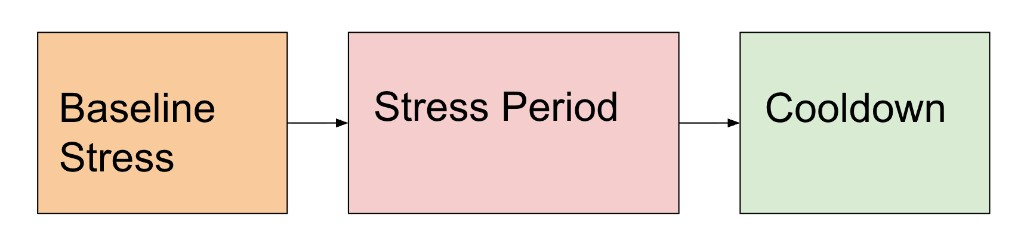
\includegraphics[width=\textwidth]{fig_concept_exp_phases.png}
  \caption{Experiment lifecycle phases for orchestrated runs: baseline (normal training and mixed load), stress (deliberate overload or fault window), and cooldown (recovery and optional scale-in).}
  \label{fig:concept-exp-phases}
\end{figure*}

%==============================================================================
\subsection{SOM Setup}
\label{subsec:som-setup}

The core detector is a \emph{Self-Organizing Map} (SOM) used as a compact nonlinear manifold model of normal system behaviour under representative operating conditions. Observations are represented as low-dimensional feature vectors derived from time-aligned infrastructure metrics (compute, memory, and storage I/O signals aggregated across Cassandra replicas). The SOM produces a Best Matching Unit (BMU) index for each observation and a scalar anomaly score derived from the map's local geometry (area around the BMU). Thresholding and temporal logic convert scores into alarms suitable for operational dashboards and mitigation experiments.

%
\subsubsection{SOM Architecture Setup}
\label{subsubsec:som-arch}

\paragraph{Topology and representation.}
The SOM is a rectangular lattice of neurons arranged in $R \times C$ cells. Each neuron $n_{r,c}$ holds a weight vector $\mathbf{w}_{r,c} \in \mathbb{R}^D$ of the same dimension $D$ as the input feature vector $\mathbf{x}(t)$ at time $t$. Neighbourhood structure is the 4-connectivity grid (north, south, east, west), used to define local neighbourhoods for training updates and for computing a local roughness map after training.

\paragraph{Input features}
Let there be $K$ Cassandra replicas indexed by $k \in \{1,\ldots,K\}$. For each sampling instant $t$, the system collects a set of scalar metrics per replica (examples: CPU usage in cores, memory working set in bytes, disk read/write throughput in bytes per second). These are aggregated into a cluster-level feature vector by averaging across replicas:
\begin{equation}
  x_j(t) \;=\; \frac{1}{K}\sum_{k=1}^{K} \tilde{x}_{j,k}(t),
  \qquad j=1,\ldots,D,
\end{equation}
where $\tilde{x}_{j,k}(t)$ denotes the $j$-th metric on replica $k$. The dimension $D$ is fixed by the metric contract (here $D{=}3$ for the triple averaged over replicas). This aggregation reduces per-node noise while preserving cluster-wide stress signatures.

\paragraph{Normalisation.}
Each feature channel is scaled to a bounded range using a per-channel maximum observed during training (capacity-style normalisation). Let $\mathrm{cap}_j > 0$ denote the scaling reference for channel $j$. The normalised vector $\mathbf{z}(t) \in [0,100]^D$ is
\begin{equation}
  z_j(t) \;=\; 100 \cdot \frac{x_j(t)}{\max\{\mathrm{cap}_j,\epsilon\}},
\end{equation}
with a small numerical floor $\epsilon$ to avoid division by zero. The same $\mathrm{cap}_j$ values are frozen after training for live inference so that scores remain comparable across runs.

\paragraph{BMU and anomaly score.}
Given $\mathbf{z}(t)$, the BMU is
\begin{equation}
  (r^\star,c^\star) \;=\; \arg\min_{(r,c)} \|\mathbf{z}(t)-\mathbf{w}_{r,c}\|_2 .
\end{equation}
A local area map $A_{r,c}$ quantifies how much the BMU neighbourhood disagrees with its neighbours (sum of absolute weight differences along edges). The anomaly score $s(t)$ is taken as $A_{r^\star,c^\star}$ (or an equivalent monotone transform of the same quantity), so that unusually rough regions of the trained map correspond to unusual operating states.

\paragraph{Operational variants.}
Two scoring variants are used in evaluation:
\begin{itemize}
  \item \textbf{UBL--NS (no smoothing):} $s_{\mathrm{NS}}(t)$ is computed directly from $\mathbf{z}(t)$.
  \item \textbf{UBL--5PtS (5-point smoothing):} $\mathbf{z}'(t)$ is a moving average of the last $K{=}5$ normalised vectors; $s_{\mathrm{5PtS}}(t)$ is computed from $\mathbf{z}'(t)$. Smoothing suppresses single-sample telemetry spikes that are not sustained across multiple polls.
\end{itemize}

%
\subsubsection{Algorithm}
\label{subsubsec:som-algorithm}

\paragraph{Training (offline bootstrap).}
Training uses a finite multiset of normal-phase samples $\{\mathbf{z}(t_i)\}_{i=1}^{N}$ collected while the cluster is under a controlled baseline workload (mixed read/write baseline) and before deliberate anomaly injection. Training proceeds for $E$ epochs with learning rate $\eta$ and neighbourhood width $\sigma$.

\begin{figure}[t]
  \centering
  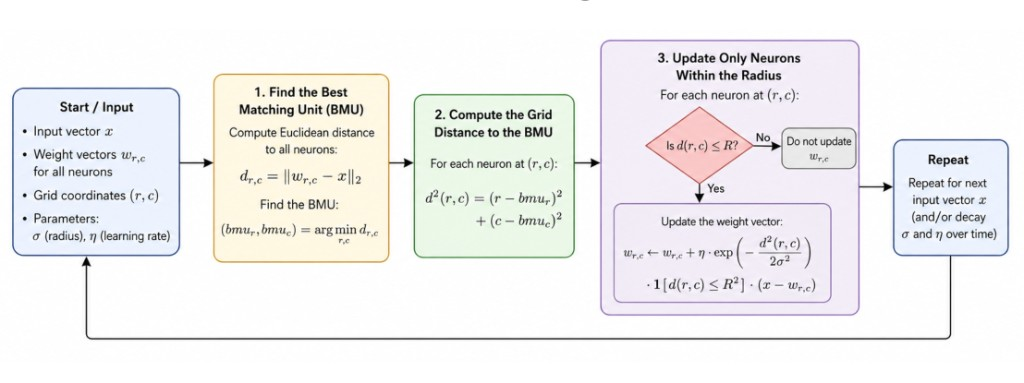
\includegraphics[width=\linewidth]{fig_concept_som_training.png}
  \caption{Conceptual SOM training loop: locate the BMU for each normalised sample, compute grid distances, and apply neighbourhood-weighted updates until convergence (with decaying $\sigma$ and $\eta$ in full implementations).}
  \label{fig:concept-som-train}
\end{figure}

\begin{algorithm}[H]
\caption{Offline SOM training (batch, random shuffle per epoch)}
\label{alg:som-train}
\KwData{Normalised samples $\{\mathbf{z}_i\}_{i=1}^{N}$; lattice size $R{\times}C$; hyperparameters $\eta,\sigma$, neighbourhood radius $h$ (integer cell steps)}
\KwResult{Trained weights $\{\mathbf{w}_{r,c}\}$; area map $\{A_{r,c}\}$; normalisation caps $\{\mathrm{cap}_j\}$}
\BlankLine
Initialise each $\mathbf{w}_{r,c}$ randomly in $[0,100]^D$\;
\For{$e = 1$ \KwTo $E$}{
  Randomly permute the training indices\;
  \ForEach{sample $\mathbf{z}$ in the permuted order}{
    Compute BMU $(r^\star,c^\star)$ by minimising $\|\mathbf{z}-\mathbf{w}_{r,c}\|_2$\;
    \ForEach{neuron $(r,c)$ within squared distance $\le h^2$ from $(r^\star,c^\star)$}{
      Compute neighbourhood kernel $g_{r,c}$ (Gaussian in grid distance)\;
      Update $\mathbf{w}_{r,c} \leftarrow \mathbf{w}_{r,c} + \eta\, g_{r,c}\,(\mathbf{z}-\mathbf{w}_{r,c})$\;
    }
  }
}
Compute area map $A_{r,c}$ from final weights using 4-neighbour edge differences\;
\Return{$\{\mathbf{w}_{r,c}\}$, $\{A_{r,c}\}$, $\{\mathrm{cap}_j\}$}\;
\end{algorithm}

\paragraph{Online scoring (live inference).}
At each poll instant $t$, the system obtains $\mathbf{x}(t)$, forms $\mathbf{z}(t)$ (or $\mathbf{z}'(t)$ for the smoothed variant), computes $(r^\star,c^\star)$ and $s(t)$, and compares $s(t)$ to a threshold $\tau$.

\begin{algorithm}[H]
\caption{Live inference with streak-based alarming}
\label{alg:som-live}
\KwData{Trained weights; caps $\mathrm{cap}_j$; threshold $\tau$; streak length $L$; optional online threshold refresh policy}
\KwResult{Score stream; alarms with timestamps and ranked causes}
\BlankLine
\While{monitoring is active}{
  Poll metrics; build $\mathbf{x}(t)$; normalise to $\mathbf{z}(t)$ (or smoothed $\mathbf{z}'(t)$)\;
  Compute BMU and score $s(t)$\;
  Optionally refresh $\tau$ from a running score distribution (controlled cadence)\;
  \eIf{$s(t) \ge \tau$}{
    increment streak counter\;
    \If{streak $\ge L$}{
      emit alarm at time $t$ with phase tag and cause list\;
    }
  }{
    reset streak counter\;
  }
}
\end{algorithm}

\begin{figure}[t]
  \centering
  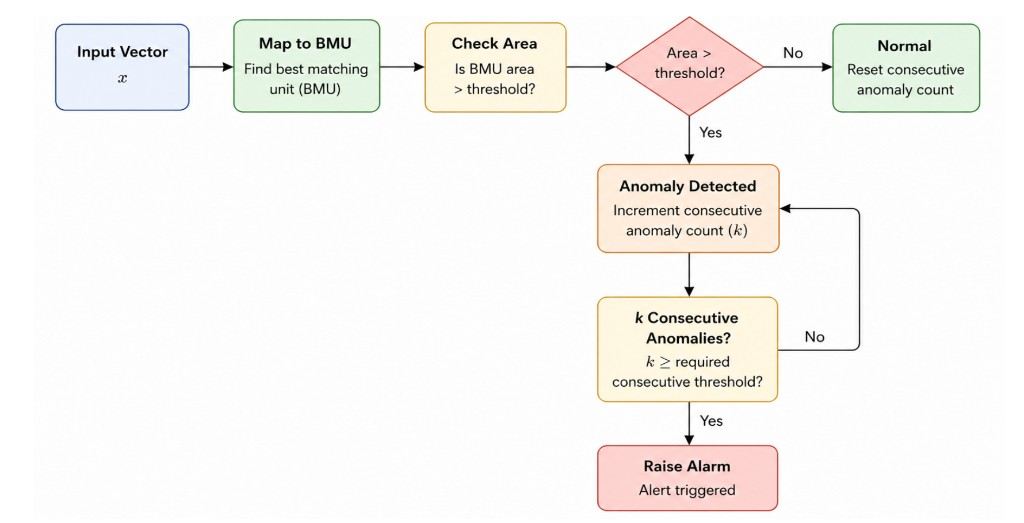
\includegraphics[width=\linewidth]{fig_concept_live_alarm_flow.png}
  \caption{Conceptual live scoring path: map each observation to a BMU, compare local map ``area'' to a threshold, count consecutive excursions, and emit an alarm only after the streak policy fires (debouncing single-scrape spikes).}
  \label{fig:concept-live-alarm}
\end{figure}

\paragraph{Cause inference (post-score).}
When an alarm fires, the system ranks candidate contributing metrics by comparing the current normalised vector to a reference normal profile (e.g., historical norms or the BMU weight vector), and returns the top-$Q$ contributors as human-readable hints.

%
\subsubsection{Hyper Parameters}
\label{subsubsec:som-hyper}

Table~\ref{tab:som-hyper} lists the principal hyperparameters, their roles, and practical guidance. The guiding principle is to balance \emph{expressiveness} (enough neurons to separate operating modes) against \emph{data sufficiency} (enough independent samples per neuron) and \emph{stability} (threshold and streak logic).

\begin{table*}[t]
\begingroup
\footnotesize
\renewcommand{\arraystretch}{1.05}
\setlength{\tabcolsep}{5pt}
\centering
\caption{SOM and decision hyperparameters (representative symbols; values are set per deployment).}
\label{tab:som-hyper}
\begin{tabularx}{\textwidth}{@{}>{\raggedright\arraybackslash}p{2.4cm}>{\raggedright\arraybackslash}p{1.6cm}>{\raggedright\arraybackslash}X@{}}
\toprule
\textbf{Symbol / name} & \textbf{Typical role} & \textbf{Meaning and importance} \\
\midrule
$R,C$ & lattice shape & Larger maps can represent more modes but need more training data and increase score variance unless regularised by training schedule. \\
$\eta$ & learning rate & Too large: unstable weights and poor generalisation; too small: underfitting / long training. Often decayed implicitly by using a moderate fixed $\eta$ with enough epochs. \\
$\sigma$ & neighbourhood width & Controls how global early updates are. Larger $\sigma$ encourages topology preservation; smaller $\sigma$ sharpens local specialisation. \\
$h$ & integer neighbourhood radius & Hard cap on grid distance for updates; prevents excessive compute on large maps. \\
$E$ & training epochs & More epochs improve fit up to a point; beyond that, risk overfitting to bootstrap noise unless bootstrap diversity is high. \\
$P$ & score percentile for $\tau$ & Sets operating trade-off: higher percentile $\Rightarrow$ fewer alarms (higher precision, lower recall) if scores are stationary; must be validated under real telemetry noise. \\
$L$ & alarm streak length & Debounces alarms: requires $L$ consecutive threshold crossings, reducing single-poll glitches at the cost of detection delay. \\
$K$ (smooth) & moving-average window & For UBL--5PtS, $K{=}5$ attenuates high-frequency noise in Tier~A signals; critical when Prometheus scrape cadence is comparable to fault dynamics. \\
$Q$ & cause list length & Larger $Q$ helps triage but can overwhelm operators; $Q{\in}[3,7]$ is typical. \\
\bottomrule
\end{tabularx}
\renewcommand{\arraystretch}{1}
\endgroup
\end{table*}

\paragraph{Missing and invalid samples.}
If mandatory Tier~A signals are absent at a poll (scrape gap, pod restart, query failure), the sample is marked invalid and \emph{must not} be silently imputed to zero; such samples are excluded from training updates and from scoring to avoid false structure in the model.

%
\subsubsection{Training Process}
\label{subsubsec:som-train-process}

\paragraph{Objective.}
Training produces a manifold summary of normal behaviour and a geometric anomaly score function suitable for streaming operation. Training is deliberately performed under a \emph{baseline workload} so that the map encodes healthy cluster dynamics (including baseline client latency behaviour), not the anomaly regimes used later for evaluation.

\paragraph{Data collection window.}
Training samples are collected over a wall-clock window long enough to:
\begin{enumerate}
  \item observe representative CPU, memory, and disk utilisation under baseline load;
  \item cover at least several Prometheus scrape intervals so temporal artefacts average out;
  \item populate the normalisation caps with stable maxima (avoid caps dominated by a single transient spike unless that transient is considered normal capacity for the lab).
\end{enumerate}

\paragraph{Bootstrap termination.}
Readiness is defined by a minimum count of valid training samples and successful construction of the map (weights initialised, trained, area map computed, threshold derived). If training cannot reach readiness within a bounded timeout, the run is considered failed for reporting purposes (prevents reporting on partially trained models).

\paragraph{Threshold calibration.}
After training, scores are computed on the bootstrap set (or on a held-out portion if a split is used). The threshold $\tau$ is set as a high percentile $P$ of those scores, encoding the assumption that most bootstrap time is normal. The percentile should be chosen to meet target false-alarm rates under baseline-only replay, then validated under stress.

\paragraph{Persistence and reproducibility.}
The trained artefact bundle includes: lattice dimensions; learned weights; area map; feature order; normalisation caps; chosen threshold; training timestamps; and summary counters (samples seen, dropped invalid samples). This enables offline replication of live scoring for ablation studies.

%
\subsubsection{Live Inference}
\label{subsubsec:live-inference}

\paragraph{Streaming loop.}
In live operation, the learner executes a periodic loop aligned to Prometheus scrape cadence (poll interval $\Delta t$). Each iteration:
\begin{enumerate}
  \item query Prometheus instant vectors for Tier~A metrics for each Cassandra replica;
  \item aggregate to $\mathbf{x}(t)$;
  \item normalise using frozen caps;
  \item optionally apply moving-average smoothing (UBL--5PtS);
  \item compute BMU and score $s(t)$;
  \item update optional online statistics (for threshold maintenance, if enabled);
  \item apply streak logic against $\tau$;
  \item append bounded retention buffers for scores and alarms (bounded deque semantics for UI/API stability).
\end{enumerate}

\paragraph{Phase tagging.}
Each scored sample and alarm is tagged with the learner \emph{phase} (\texttt{normal}, \texttt{load}, \texttt{chaos}, \texttt{cooldown}) driven by the orchestration state machine. Phase tags are essential for separating baseline drift from anomaly windows in evaluation.

\paragraph{Operational latency.}
End-to-end detection latency includes: Prometheus scrape delay, PromQL evaluation time, network RTT, Python processing, and alarm debounce ($L$). Reported scoring latency should be interpreted as client-side processing time, not full control-loop latency to mitigation actuation.

%
\subsubsection{Cause Inference Process}
\label{subsubsec:cause-inference}

\paragraph{Goal.}
When an alarm triggers, operators need a compact explanation in the native units of observability (which metric channels deviated). Cause inference is a \emph{post-hoc attribution} step: it does not change the score, but ranks contributors.

\paragraph{Method (conceptual).}
Let $\mathbf{z}(t)$ be the normalised observation and $\mathbf{v}$ a reference vector (e.g., the BMU weight $\mathbf{w}_{r^\star,c^\star}$ or a long-run median profile). Rank channels $j$ by absolute deviation $|z_j(t)-v_j|$, optionally weighted by channel reliability (variance, missingness rate). Return the top-$Q$ channel names with their deviations and directions (high vs low).

\begin{figure}[t]
  \centering
  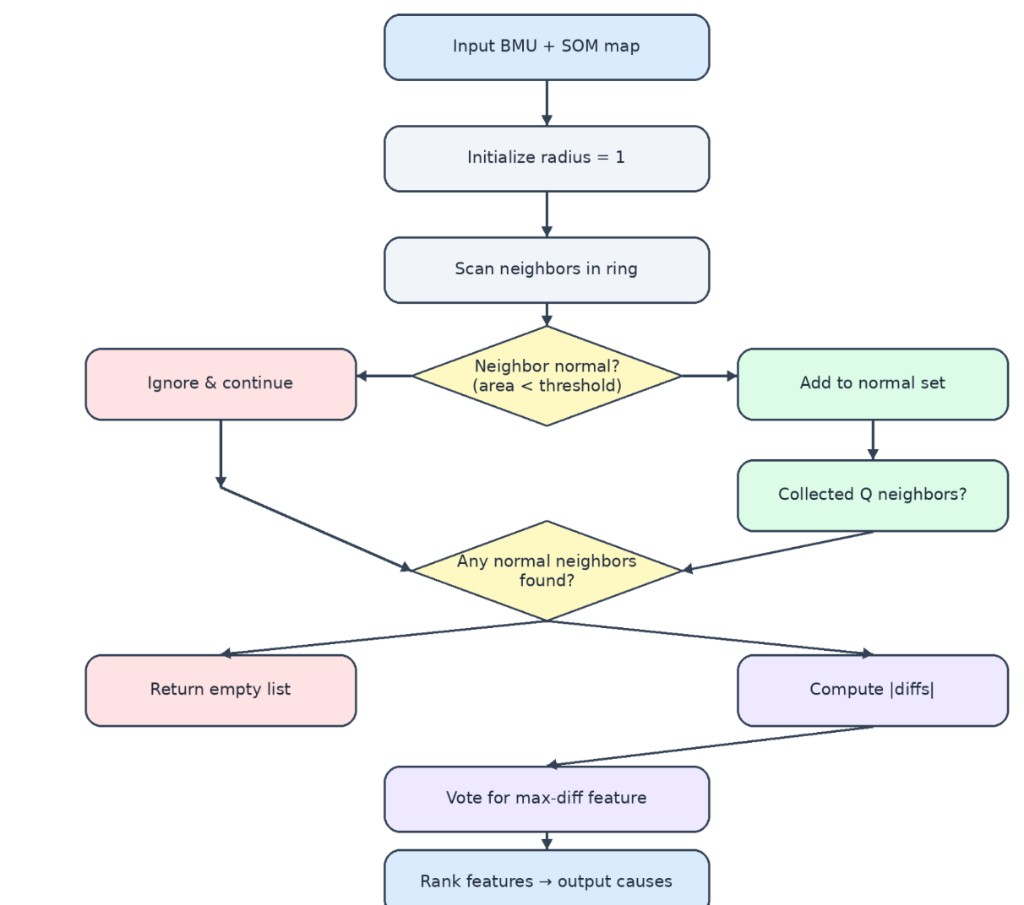
\includegraphics[width=\linewidth]{fig_concept_cause_inference.png}
  \caption{Conceptual cause inference: expand around the BMU on the trained map, collect normal-reference neighbours inside a radius budget, compare channel-wise magnitudes, and rank the largest deviations as candidate causes.}
  \label{fig:concept-cause}
\end{figure}

\paragraph{Interpretation caveats.}
\begin{itemize}
  \item Causes are \emph{correlational}: a high-ranked disk metric may reflect compaction, client write amplification, or OS page cache effects.
  \item Aggregation across replicas can hide single-node hotspots; if hotspot detection is required, rank per-replica deviations before aggregation.
\end{itemize}

%==============================================================================
\subsection{Architecture Setup}
\label{subsec:arch-setup}

%
\subsubsection{SOM Architecture Setup}
\label{subsubsec:arch-som}

The SOM learner is deployed as a stateless(ish) microservice behind a ClusterIP Service: it exposes health, training status, phase control, score stream, alarms, and a metrics endpoint for Prometheus scraping. It reads telemetry from the in-cluster Prometheus (or a reachable Prometheus base URL), not directly from node agents, preserving a clean separation of concerns: \emph{collection/scrape} vs \emph{model inference}.

%
\subsubsection{K3S and Kubernetes Setup}
\label{subsubsec:k3s}

\paragraph{k3s role.}
k3s is used as a lightweight CNCF-compliant Kubernetes distribution suitable for lab clusters on constrained VMs. It provides the standard control plane API (scheduling, controllers) and CNI-based pod networking, while reducing operational overhead compared to full kubeadm clusters.

\begin{figure}[t]
  \centering
  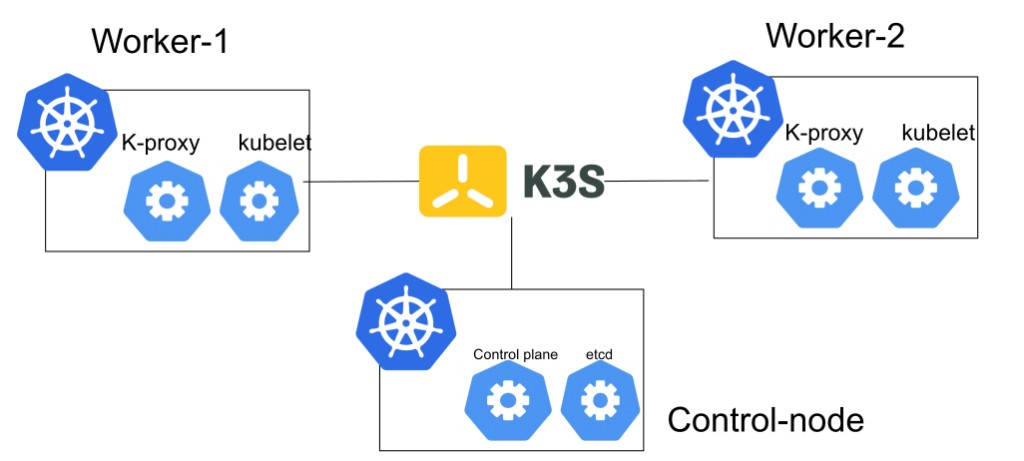
\includegraphics[width=\linewidth]{fig_concept_k3s_topology.png}
  \caption{Conceptual \texttt{k3s} deployment: control plane components and workers share a compact footprint suitable for multi-VM lab hosts.}
  \label{fig:concept-k3s}
\end{figure}

\paragraph{Cluster shape.}
The lab topology uses one control-plane node and multiple worker nodes. Worker count must be sufficient to place at least three Cassandra replicas on distinct hosts for realistic failure domains.

\paragraph{kubeconfig and access.}
Administrators interact via \texttt{kubectl} using a kubeconfig whose server endpoint matches the control-plane API address (not loopback unless port-forwarded). For laptop-driven orchestration, reliable port-forwards or VPN routes are required because the orchestrator uses HTTP to Services.

\paragraph{Storage implications.}
Default lab storage classes (e.g., local-path on k3s) bind volumes to nodes. StatefulSets with persistent volumes therefore interact with scheduling: a pod may become unschedulable if node affinity and volume topology disagree. Operational playbooks must include PVC lifecycle steps when node labels or placement constraints change.

%
\subsubsection{Node Architecture}
\label{subsubsec:node-arch}

\paragraph{Control plane node.}
Hosts Kubernetes control components and \emph{non-data-plane} services that are convenient to co-locate with the API server (e.g., chaos control plane, monitoring stack depending on pinning policy). Pinning monitoring to a dedicated node reduces interference with Cassandra workers.

\paragraph{Worker nodes.}
Host Cassandra StatefulSet pods, NoSQLBench job pods, and optionally simulator pods. Anti-affinity or explicit hostname lists are used to spread Cassandra replicas across workers.

\begin{figure*}[t]
  \centering
  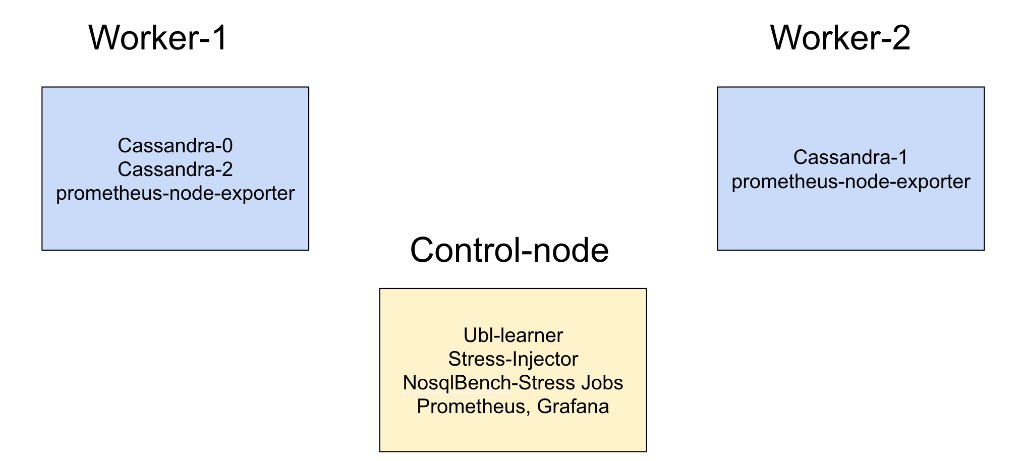
\includegraphics[width=\textwidth]{fig_concept_node_pinning.png}
  \caption{Representative lab placement: Cassandra replicas and node exporters on workers; learner, stress injector, NoSQLBench jobs, and the observability stack on the control-oriented node (exact labels depend on the deployed manifest).}
  \label{fig:concept-nodes}
\end{figure*}

\paragraph{Network.}
Pod-to-pod traffic uses cluster DNS names. Cassandra uses a headless service for per-pod DNS ($\texttt{cassandra-0.cassandra.\dots}$) while clients may target a non-headless service for load-balanced first contact.

%
\subsubsection{Monitoring Setup: Prometheus and Grafana}
\label{subsubsec:monitoring}

\paragraph{Prometheus Operator stack.}
Monitoring is deployed via Helm chart \texttt{kube-prometheus-stack}, which installs Prometheus, Alertmanager, Grafana, ServiceMonitors/PodMonitors CRDs, and default kubelet/cAdvisor scrapes. This provides a unified metrics plane for both infrastructure (CPU/memory/disk/network) and application metrics (JMX exporters, learner metrics, simulator metrics).

\paragraph{PodMonitors.}
Application components expose Prometheus text on \texttt{/metrics} (or a dedicated port). PodMonitors select pods by labels and scrape on an interval (e.g., 15s). This is the mechanism by which NoSQLBench histostat exporter sidecars become first-class Prometheus series without embedding a Prometheus client inside Cassandra itself.

\paragraph{Grafana.}
Grafana is provisioned with a lab dashboard that overlays:
\begin{itemize}
  \item per-pod CPU/memory/network time series (container metrics),
  \item client-side latency percentiles from stress tools (where available),
  \item scenario markers (load profile switches) as annotations.
\end{itemize}

\begin{figure*}[t]
  \centering
  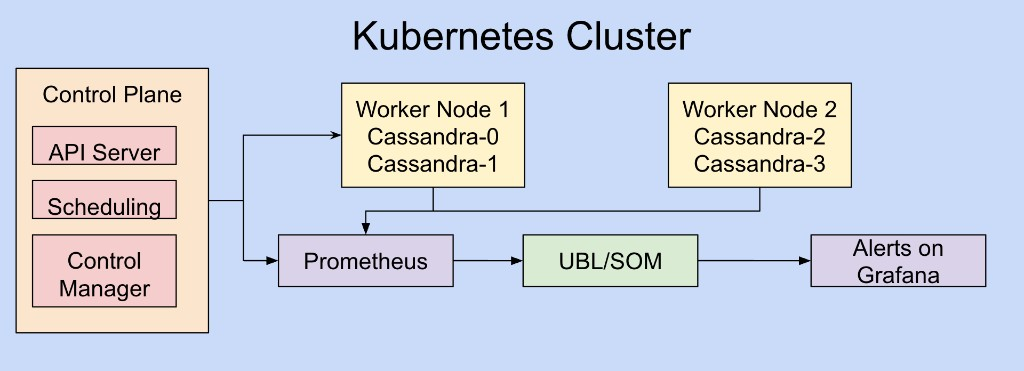
\includegraphics[width=\textwidth]{fig_concept_k8s_observability.png}
  \caption{Kubernetes cluster view for observability: workers host Cassandra data pods; Prometheus scrapes infrastructure and application targets; the UBL/SOM learner consumes series and surfaces alarms through Grafana dashboards.}
  \label{fig:concept-k8s-obs}
\end{figure*}

%==============================================================================
\subsection{Stress Injector Setup}
\label{subsec:stress}

%
\subsubsection{Stress Injector Architecture Setup}
\label{subsubsec:stress-arch}

\paragraph{Purpose.}
The stress injector is a control-plane service that translates high-level experiment profiles into concrete cluster actions: primarily \emph{ephemeral Kubernetes Jobs} that run NoSQLBench (NB5) against Cassandra, plus optional auxiliary faults (CPU burn inside a Cassandra container, network policies, StatefulSet replica scaling).

\begin{figure*}[t]
  \centering
  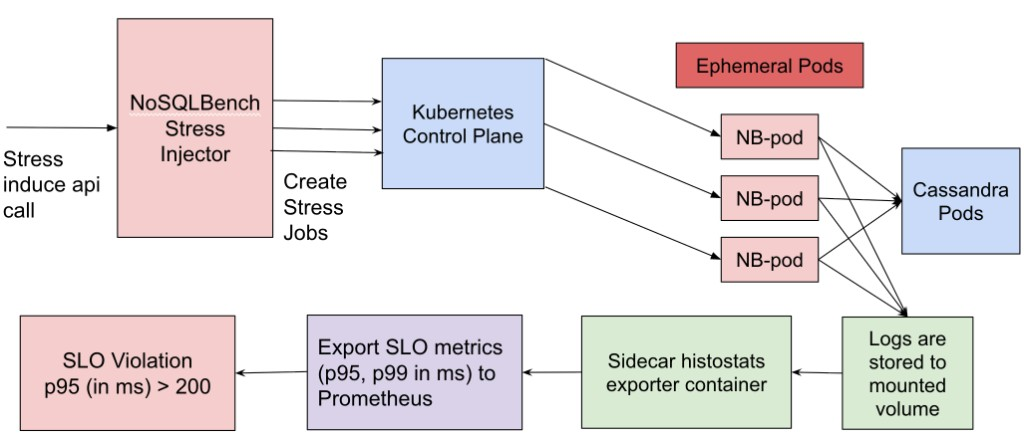
\includegraphics[width=\textwidth]{fig_concept_stress_slo_pipeline.png}
  \caption{Stress injection and SLO instrumentation path: API-driven injector creates ephemeral NoSQLBench jobs, workloads hit Cassandra, histostats flow through a sidecar exporter into Prometheus, and PromQL rules encode client-side SLO breaches (e.g., $p_{95}$ latency).}
  \label{fig:concept-stress-slo}
\end{figure*}

\paragraph{End-to-end NoSQLBench path (conceptual).}
\begin{enumerate}
  \item \textbf{Orchestration command:} an operator script triggers an experiment timeline: reset $\rightarrow$ baseline training window $\rightarrow$ chaos window $\rightarrow$ cooldown. It drives three APIs: simulator load level, learner phase, and stress injector profile start/stop.
  \item \textbf{Profile dispatch:} the injector receives a profile name and parameters (duration, threads, parallelism, replication factor). It maps the profile to a NoSQLBench \emph{scenario document} (YAML) that defines schema creation, ramp-up, and main workload phases.
  \item \textbf{Parallelism model:} parallelism is expressed as $J$ independent Jobs (distinct pods). Each Job runs an isolated NB process with its own thread pool, multiplying client-side concurrency and TCP connection diversity.
  \item \textbf{Keyspace isolation:} each Job uses a distinct keyspace token derived from its Job name to avoid cross-job schema collisions while still hitting the same physical cluster.
  \item \textbf{Cassandra contact:} NB is configured with a \texttt{hosts=} contact list. The default lab configuration uses a stable DNS service name that selects Cassandra pods; the CQL driver discovers the full ring topology after the first contact.
  \item \textbf{Optional Prometheus push:} NB can be configured to push client metrics to a metrics sink (VictoriaMetrics-compatible import or Pushgateway-style endpoints). This path is orthogonal to histostats-on-PVC.
  \item \textbf{Histostats durability path:} when enabled, each Job pod mounts a shared PVC path. NB writes HDR histogram statistics to \texttt{hdrstats.csv} under a per-job directory on a fixed interval. A lightweight \emph{sidecar} container in the same pod reads the CSV and serves Prometheus exposition format on \texttt{/metrics}.
  \item \textbf{Prometheus scrape:} a PodMonitor selects NB Job pods by label and scrapes the sidecar port periodically, ingesting \texttt{nosqlbench\_histostat\_p95\_ms} and \texttt{nosqlbench\_histostat\_p99\_ms} time series (tagged by operation tag, job name, profile).
  \item \textbf{Grafana visualisation:} dashboard panels query these series (typically \texttt{max by (job)} with \texttt{tag="execute"}) to show client latency percentiles aligned in time with infrastructure saturation panels.
  \item \textbf{Ephemeral completion:} Jobs are configured with no retries and a post-finish TTL so completed pods do not accumulate indefinitely. The PVC retains histostat files for post-run inspection even after pods disappear.
\end{enumerate}

\paragraph{Why sidecar + PVC.}
NoSQLBench histostats are file-oriented time series logs. Kubernetes pod logs alone are insufficient for reliable post-run analysis under churn. Persisting \texttt{hdrstats.csv} on a PVC decouples durability from pod lifetime, while the sidecar decouples \emph{Prometheus exposition} from the NB Java process.

%
\subsubsection{How do we inject faults}
\label{subsubsec:faults}

Fault injection is split into two families:

\paragraph{(A) Load faults via NoSQLBench.}
These are not bit flips; they are sustained CQL workloads that change partition access patterns, payload sizes, and write/read ratios. Examples include: mixed baseline, write-only concurrency spikes, wide-row compaction pressure, and large-blob inserts.

\paragraph{(B) Infrastructure faults outside NB.}
Examples include:
\begin{itemize}
  \item \textbf{CPU starvation inside a Cassandra pod:} execute a tight computational loop inside the Cassandra container for a bounded duration to reduce available CPU for compaction, flushing, and request handling without changing CQL workload parameters.
  \item \textbf{Replica count manipulation:} temporarily scale the Cassandra StatefulSet to fewer replicas to create a capacity bottleneck, then restore.
  \item \textbf{Network impairment:} apply Kubernetes NetworkPolicies or traffic shaping (if used in a given profile) to increase latency/packet loss between namespaces or pods.
\end{itemize}

Faults are orchestrated with explicit start/stop boundaries so evaluation can align alarms to a known chaos window.

%
\subsubsection{SLO Metrics setup}
\label{subsubsec:slo}

\paragraph{Definition.}
Service-level objectives (SLOs) for the lab are expressed on \emph{client-side} latency percentiles for the execute path (e.g., $p_{95}$ and $p_{99}$ in milliseconds). These are preferred over raw CPU metrics as an externally meaningful user pain proxy.

\paragraph{Acquisition paths.}
Two complementary acquisition modes exist:
\begin{enumerate}
  \item \textbf{Pull (recommended for Prometheus):} NB histostats CSV $\rightarrow$ sidecar exporter $\rightarrow$ \texttt{/metrics} $\rightarrow$ Prometheus scrape $\rightarrow$ Grafana.
  \item \textbf{Push (optional):} NB built-in reporter pushes time series to a metrics sink; useful when scrape targets are short-lived and push is operationally simpler. Push endpoints must accept the exposition format NB emits in the deployed version.
\end{enumerate}

\paragraph{SLO violation rule (instantaneous).}
At time $t$, let $p_{95}(t)$ be the scraped $p_{95}$ in ms. Given threshold $\theta$, an instantaneous violation indicator is
\begin{equation}
  V(t) = \mathbb{I}\big[p_{95}(t) > \theta\big].
\end{equation}
Operational evaluation often uses a \emph{pending window} $W$: an alarm at $t_a$ is treated as a true positive if a violation occurs within $(t_a, t_a+W]$ (lead-time semantics).

%
\subsubsection{Stress Profiles}
\label{subsubsec:profiles}

Stress profiles are reproducible bundles of: (i) NB scenario YAML, (ii) default thread counts, (iii) parallelism, (iv) payload distributions, and (v) optional non-NB faults. Table~\ref{tab:profiles} summarises the profiles used in the lab narrative.

\FloatBarrier
\Needspace{22\baselineskip}
\begin{table}[H]
\centering
\renewcommand{\arraystretch}{1.15}
\caption{Stress profiles}
\label{tab:profiles}
\begin{tabularx}{\linewidth}{@{}>{\raggedright\arraybackslash}p{3.5cm}>{\raggedright\arraybackslash}X@{}}
\toprule
\textbf{Profile} & \textbf{Induced behaviour (Cassandra perspective)} \\
\midrule
Baseline mixed &
Creates RF=3 keyspace and table; generates random partition/clustering keys in a bounded hash space; executes 50/50 inserts and single-partition reads at LOCAL\_ONE-like consistency; measures normal latency spread. \\
Short CPU spike &
Runs the same baseline CQL load while one Cassandra node executes a CPU burn-in loop for a short wall interval; isolates CPU scheduling effects from workload-shape changes. \\
CPU pressure (write spike) &
Write-only high-rate inserts across a large hash space with many client threads across multiple parallel jobs; stresses coordinator/replica CPU and write paths. \\
Disk pressure (large payloads) &
Insert-only workload with large binary payloads (hundreds of KiB per row) and high concurrency; stresses memtable growth, flush frequency, and disk write bandwidth. \\
Compaction pressure (concentrated keys) &
Insert-only workload concentrated in a smaller partition key space with very few clustering values; increases overlap across SSTables and amplifies compaction read/write amplification. \\
\bottomrule
\end{tabularx}
\renewcommand{\arraystretch}{1}
\end{table}
\FloatBarrier

%==============================================================================
\subsection{Mitigation}
\label{subsec:mitigation}

\paragraph{Goal.}
Demonstrate a closed-loop response: when the system detects sustained stress/fault conditions, increase Cassandra capacity (scale out), wait for recovery signals, then scale back in.

\begin{figure*}[t]
  \centering
  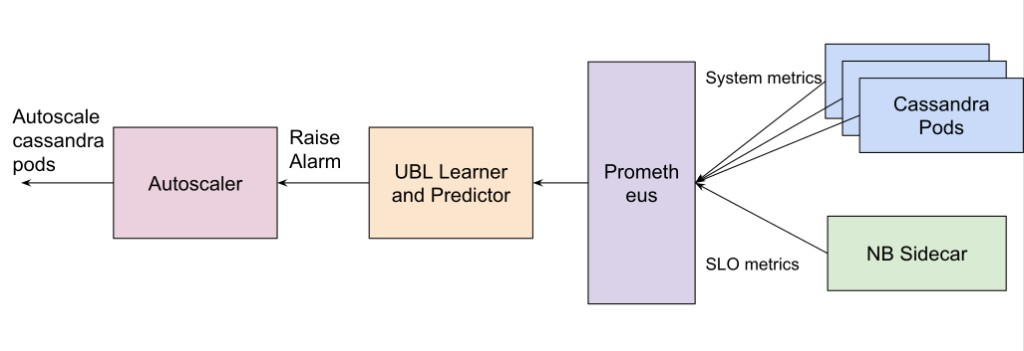
\includegraphics[width=\textwidth]{fig_concept_data_plane_mitigation.png}
  \caption{Closed-loop data plane: Cassandra system metrics and NoSQLBench-derived SLO series feed Prometheus; the UBL learner raises alarms into an autoscaler hook that can scale the Cassandra StatefulSet when policy conditions are met.}
  \label{fig:concept-mitigation-plane}
\end{figure*}

\paragraph{Actuation mechanism.}
Mitigation uses Kubernetes API scaling of the Cassandra StatefulSet replica count (e.g., $3 \rightarrow 4 \rightarrow 3$). This is demo-grade: it does not replace production procedures (bootstrap, repair, decommission) but is sufficient to show scheduling of a new replica on spare worker capacity.

\paragraph{Triggering policy (two-channel).}
A mitigation daemon can scale out on either:
\begin{itemize}
  \item \textbf{Learner alarms:} require a streak of consecutive chaos-phase alarms in chronological order after a watch start timestamp (reduces false scaling on stale alarms retained in bounded buffers).
  \item \textbf{Prometheus SLO signal:} require the PromQL-defined SLO signal to remain in a bad band for a sustained interval before scaling out (reduces flapping).
\end{itemize}

\paragraph{Scale-in gating (hysteresis).}
Scale-in waits until the PromQL SLO signal remains in an OK band for a sustained window (hysteresis), preventing immediate scale-down while the cluster is still unstable.

\paragraph{Operational prerequisites.}
A spare worker node (or allocatable capacity) must exist so the new StatefulSet ordinal can schedule; otherwise scale-out stalls in Pending. Port-forward paths must expose Prometheus query API to the mitigation script if it runs off-cluster.

%==============================================================================
\subsection{Evaluation}
\label{subsec:evaluation}

This subsection defines the counting semantics used in experiment reports. Let:
\begin{itemize}
  \item $t^{\mathrm{chaos}}_{\mathrm{start}}$ and $t^{\mathrm{chaos}}_{\mathrm{stop}}$ bound the injected anomaly window (fault start/stop).
  \item Each learner alarm is an event with timestamp $t^{\mathrm{alarm}}$.
  \item SLO breach events have timestamps $\{t^{\mathrm{slo}}_m\}$ derived from client latency thresholds (possibly smoothed by scrape cadence).
  \item $W$ denotes a pending/lead-time window (seconds), aligned with offline ROC plots such as CPU ROC ($W{=}10$s).
\end{itemize}

\subsubsection*{Alarm--SLO alignment for true/false positives}

\paragraph{True positive count (\texttt{Ntp}).}
An alarm at time $t^{\mathrm{alarm}}$ counts as a true positive if a genuine anomaly effect (operationalised as an SLO breach) occurs within the forward window $(t^{\mathrm{alarm}}, t^{\mathrm{alarm}}+W]$:
\begin{equation}
  \exists\, t^{\mathrm{slo}} \in (t^{\mathrm{alarm}}, t^{\mathrm{alarm}}+W] \;\text{ such that the breach definition holds at } t^{\mathrm{slo}}.
\end{equation}
This matches the narrative alarm raised; anomaly happens within window.

\paragraph{False positive count (\texttt{Nfp}).}
An alarm counts as a false positive if \emph{no} qualifying SLO breach occurs within $(t^{\mathrm{alarm}}, t^{\mathrm{alarm}}+W]$:
\begin{equation}
  \nexists\, t^{\mathrm{slo}} \in (t^{\mathrm{alarm}}, t^{\mathrm{alarm}}+W] \text{ satisfying the breach condition.}
\end{equation}
This matches alarm raised; anomaly does not happen within window.

\paragraph{False negative count (\texttt{Nfn}).}
A false negative corresponds to an SLO breach event without a preceding alarm in the allowed lead window. Concretely, for a breach at $t^{\mathrm{slo}}$, there should have existed an alarm $t^{\mathrm{alarm}}$ such that $t^{\mathrm{alarm}} < t^{\mathrm{slo}} \le t^{\mathrm{alarm}}+W$. If no such alarm exists, count one false negative:
\begin{equation}
  \text{\texttt{Nfn}} \mathrel{+}= 1 \quad \text{for breaches lacking qualifying prior alarms.}
\end{equation}
This matches anomaly happens; no prior alarm raised when prior is interpreted in the lead-time sense above.

\paragraph{True negative count (\texttt{Ntn}).}
During normal operation intervals (outside the forward influence of alarms and outside labelled anomaly windows), the system should remain quiet. Operationally, \texttt{Ntn} counts time buckets or evaluation ticks where neither an alarm nor a breach condition is present, depending on the evaluation discretisation. This matches normal period; no prior alarm raised when the evaluation frame is defined as pre-alarm normalcy.

\subsubsection*{Lead time}

\paragraph{Definition.}
For a matched alarm--breach pair, \emph{lead time} quantifies how early the alarm precedes the SLO breach. Let $t^{\mathrm{alarm}}$ be the first alarm in a cluster of alarms that precedes a breach at $t^{\mathrm{slo}}$ within window $W$. Lead time is
\begin{equation}
  \mathrm{LT} = t^{\mathrm{slo}} - t^{\mathrm{alarm}}.
\end{equation}
The user-facing definition first SLO breach timestamp minus first alarm timestamp corresponds to pairing the earliest breach in the post-alarm window with the triggering alarm (policy choices exist if multiple breaches occur).

\subsubsection*{ROC/AUC and accuracy (offline)}

\paragraph{ROC.}
Receiver Operating Characteristic curves sweep a score threshold $\tau$ and plot TPR vs FPR at each threshold using tick-level (or sample-level) labels derived from the pending breach definition within window $W$.

\paragraph{AUC.}
Area Under the Curve summarises ranking quality across thresholds; it is threshold-free unlike accuracy.

\paragraph{Accuracy.}
Accuracy requires a single chosen threshold \emph{and} class prevalence; it cannot be inferred from an ROC curve alone without specifying both.

\subsubsection*{Run-level reporting vs tick-level ROC}

Run-level summaries that count alarms inside a global chaos window (fault start/stop) are useful for operational acceptance gates but are \emph{not} identical to ROC-based definitions unless alarms and breaches are discretised consistently. Reports should explicitly state which definition is used for each table.

%--

% \begin{figure}
%     \centering
%     \includegraphics[width=1\linewidth]{diagram/arch-diagram.png}
%     \caption{Proposed Approach}
%     \label{fig:placeholder}
% \end{figure}



% In this study, a framework for anomaly detection has been proposed, specifically designed for distributed microservice-based systems, where replicas of microservices are containerized using Docker services. A unified representation of various sources of telemetry, such as system metrics, application metrics, system call traces, and structured logs, will be integrated into a single behavioral representation, which will then be utilized for unsupervised machine learning and fault detection.

% For this study, a microservice-based architecture will be designed and implemented, comprising a multi-tiered architecture, where microservices are deployed across various replicas of containers. To simulate various types of anomalies, a controlled perturbation mechanism will be implemented, which will introduce reproducible anomalies to simulate diverse operating conditions. To achieve this, a distributed ingestion layer will be designed to collect various types of telemetry, such as resource metrics, application metrics, traces of interactions with the Linux kernel, and structured logs. 

% Resource metrics define various types of physical resources, whereas application metrics define various types of application-specific metrics, including request rates, latency, thread pool saturation, and connection counts. Simultaneously, a tracing module will be designed to capture system call traces, which will then be converted into System Call Frequency Distribution vectors. Furthermore, a module for structured logs will be designed to capture various types of log information, including template identifiers and severity.

% This fused representation will then mapped onto a three-dimensional self-organising map (SOM) topology that extends the original UBL framework \cite{10.1145/2371536.2371572}. By increasing the size of the connectivity groups, the mapping improves the representation of the high-dimensional space defined by the multimodal signals and reduces the distortion of the representation in a planar space. Clusters in the topology correspond to the typical operational regimes, while any deviations from these clusters indicate anomalous system behaviour. This will maintain the interpretability of the system while increasing the ability to detect subtle changes in system behaviour that can only be captured by the correlation of resource consumption and execution intent/semantic indicators.

% \subsection{Evaluation}

% Fault scenarios will be constructed based on realistic system degradation in the operational context of a containerized system. This includes resource thrashing, thread pool misconfiguration, memory allocation faults at control group boundaries, burst traffic, database queries that extend over long periods of time and amplify latency, inter-process communication faults that appear as synchronisation or socket errors, packet loss and network instability, connection leaks, memory leaks, distributed denial of service, context switching, garbage collector stalls, domain resolution faults, retry cascades, and file synchronisation delays from buffering and flushing. 

% These fault scenarios perturb the signals across the various modalities, allowing the accuracy of the detection to be evaluated. By using this approach, the framework can evaluate the ability of the enriched telemetry fusion and higher-dimensional mapping to correctly discriminate between nominal and anomalous system behaviour in the context of a distributed containerised system.

\section{Results and Discussion}
\label{sec:results}

This section summarises quantitative outcomes from the Cassandra--\texttt{k3s} lab described in Section~\ref{sec:methodology}: offline scoring quality, configuration ablations, training cost, lead-time behaviour under alternative streak policies, post-hoc cause attribution under three stress families, and a controlled mitigation run against a client-side $p_{95}$ SLO band. All plots and tables report \emph{our} measurements only; file names expected under \texttt{figures/} are listed in \texttt{figures/README.txt} alongside the \LaTeX{} source.

%------------------------------------------------------------------------------
\subsection{Offline detection quality (CPU pressure, pending window)}
\label{subsec:res-roc}

We first evaluate tick-level ranking quality when labels are derived from the pending-window semantics with $W{=}10$\,s (Section~\ref{subsec:evaluation}). Figure~\ref{fig:cpu-roc-w10} contrasts two operationalisations of the same SOM backbone: \textbf{UBL--5PtS} (five-sample moving average on normalised inputs before BMU scoring) versus \textbf{UBL--NS} (no input smoothing).

UBL--5PtS reaches an area under the ROC curve (AUC) of \textbf{0.795}, indicating usable separation between alarm-like scores and breach events inside the chosen window. UBL--NS attains \textbf{0.496}, i.e.\ performance indistinguishable from random threshold sweeps for this configuration. The gap supports the design choice in our pipeline: short-horizon smoothing attenuates single-scrape telemetry spikes that otherwise distort distances to the trained lattice without requiring extra labelled data.

\begin{figure}[t]
  \centering
  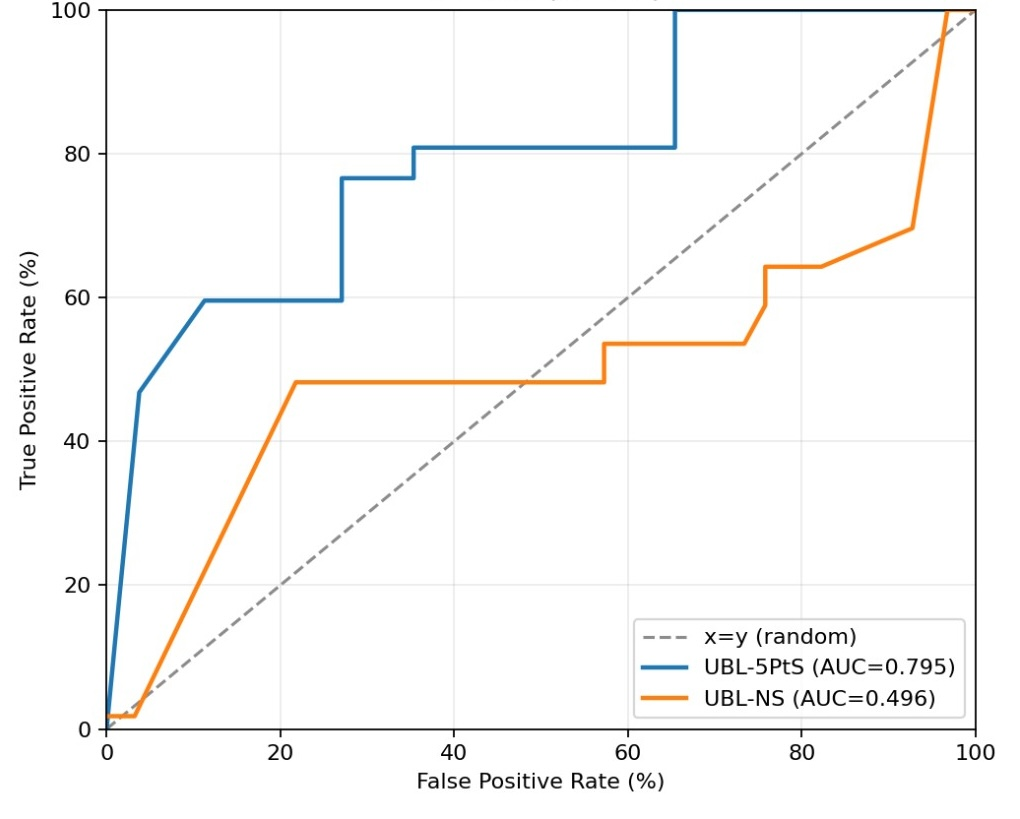
\includegraphics[width=\linewidth]{fig_cpu_roc_w10.png}
  \caption{CPU-condition ROC with pending window $W{=}10$\,s: UBL--5PtS (AUC $=0.795$) versus UBL--NS (AUC $=0.496$).}
  \label{fig:cpu-roc-w10}
\end{figure}

%------------------------------------------------------------------------------
\subsection{Lattice and decision hyperparameter ablations}
\label{subsec:res-ablation}

Table~\ref{tab:ubl-ablation-cpu} reports accuracy on the CPU-pressure scenario while varying one family of hyperparameters at a time (map side length, neighbourhood width used in the local roughness map, and percentile-derived alarm threshold). The best single configuration in this sweep is a \textbf{$32{\times}32$} map, neighbourhood size \textbf{4}, and threshold \textbf{85}, each coinciding with peak accuracy \textbf{80.82\%}.

Map size exhibits a mild inverted-U: both $25{\times}25$ and $40{\times}40$ trail $32{\times}32$, suggesting either insufficient capacity or excess variance when the lattice is too large relative to the effective diversity of bootstrap windows. Neighbourhood size is comparatively stable ($3$--$5$ within a fraction of a percent), which is desirable for deployment tuning. Threshold choice is the most brittle knob in this table: moving from $85$ to $90$ costs nearly ten absolute percentage points, while $80$ also underperforms---consistent with percentile thresholds acting as implicit false-alarm versus miss trade-offs on finite runs.

\begin{table*}[t]
  \centering
  \footnotesize
  \caption{UBL ablation on CPU-pressure accuracy (\%). Best per group in bold.}
  \label{tab:ubl-ablation-cpu}
  \begin{tabular}{@{}llr@{}}
    \toprule
    \textbf{Group} & \textbf{Setting} & \textbf{Accuracy} \\
    \midrule
    \multirow{3}{*}{Map (grid)} & $25{\times}25$ & 78.94 \\
    & $\mathbf{32{\times}32}$ & \textbf{80.82} \\
    & $40{\times}40$ & 78.26 \\
    \midrule
    \multirow{3}{*}{Neighbourhood size} & 3 & 80.36 \\
    & \textbf{4} & \textbf{80.82} \\
    & 5 & 80.48 \\
    \midrule
    \multirow{3}{*}{Threshold} & 80 & 76.16 \\
    & \textbf{85} & \textbf{80.82} \\
    & 90 & 70.98 \\
    \bottomrule
  \end{tabular}
\end{table*}

%------------------------------------------------------------------------------
\subsection{Offline training time}
\label{subsec:res-train-time}

Figure~\ref{fig:train-time} compares wall-clock offline training time for the deployed SOM trainer versus a $k$-NN baseline on the same feature matrix. SOM training takes \textbf{0.562\,s} compared to \textbf{0.248\,s} for $k$-NN in this configuration. Both are sub-second on our bootstrap slice, so the comparison should be read as a sanity check on interactive iteration rather than a large-scale benchmark: absolute seconds will grow with sample count, lattice size, and Python/BLAS overhead. The practical takeaway for our project is that SOM training remains lightweight enough to repeat during lab sessions while still providing a nonparametric manifold structure that $k$-NN does not encode explicitly.

\begin{figure}[t]
  \centering
  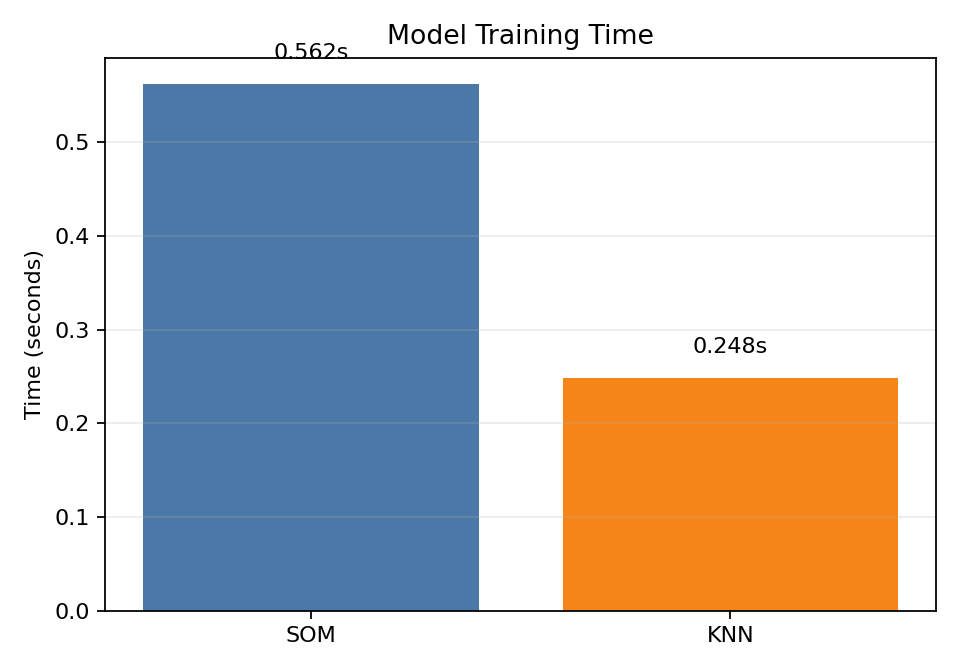
\includegraphics[width=\linewidth]{fig_training_time_som_knn.png}
  \caption{Offline training time: SOM vs.\ $k$-NN (seconds).}
  \label{fig:train-time}
\end{figure}

%------------------------------------------------------------------------------
\subsection{Lead time by stress family and streak length}
\label{subsec:res-lead}

\paragraph{Stress-family averages.}
Figure~\ref{fig:avg-lead} summarises mean lead time (first qualifying alarm to first SLO breach in the evaluation harness) aggregated by induced stress family. Disk-heavy profiles exhibit the longest average lead time (\textbf{15.65\,s}), followed by CPU-centric stress (\textbf{9.50\,s}). Memory-labelled runs register \textbf{0.00\,s} mean lead in this aggregation, which signals a mismatch between how ``memory pressure'' manifests in container-level telemetry versus how the SLO breach clock fires for those runs (for example, breaches aligned with the same scrape as the first alarm, or memory stress rarely crossing the SLO rule while still moving scores). The disk and CPU numbers are the primary carriers of early-warning behaviour in our current scenario matrix.

\begin{figure}[t]
  \centering
  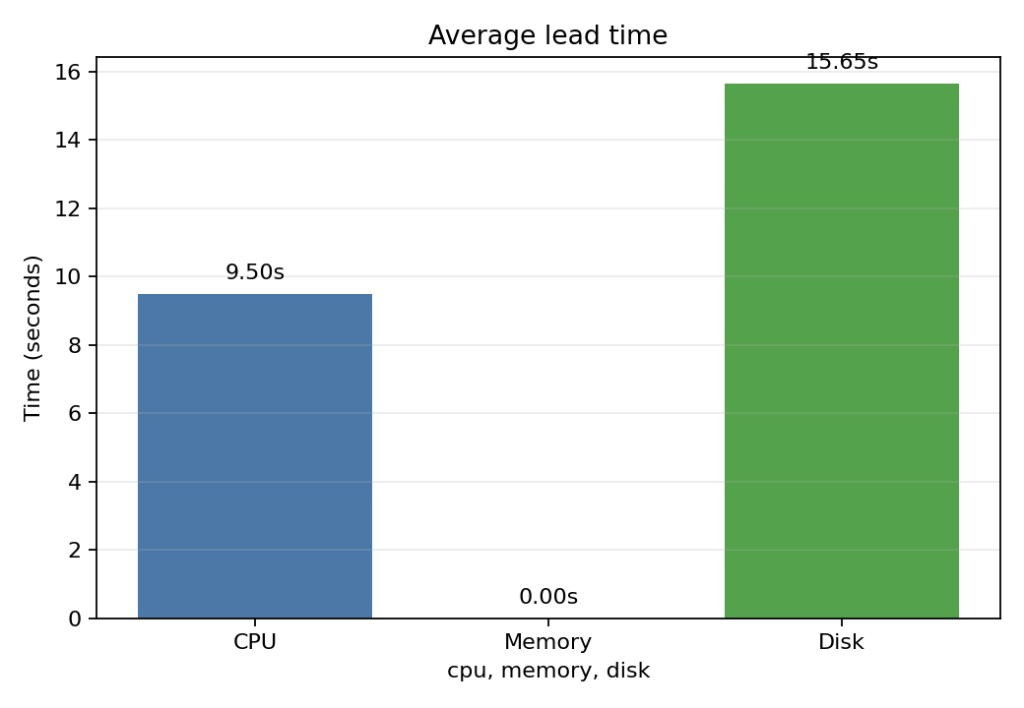
\includegraphics[width=\linewidth]{fig_avg_lead_time.png}
  \caption{Average lead time (seconds) by stress family (CPU, memory, disk).}
  \label{fig:avg-lead}
\end{figure}

\paragraph{Streak length $K$.}
Figure~\ref{fig:lead-ablation-k} ablates the consecutive-alarm requirement $K$ against the same lead-time statistic. For $K\in\{2,3\}$, lead times remain high (\textbf{27.83\,s} and \textbf{27.28\,s}), indicating that accepting almost every threshold crossing as an alarm preserves a long warning horizon for the CPU scenarios used in this ablation. Increasing debounce to $K{=}5$ collapses lead time to \textbf{9.50\,s}; $K{=}7$ yields \textbf{8.42\,s} with diminishing further returns.

The elbow between $K{=}3$ and $K{=}5$ is the operational story: aggressive debouncing removes many borderline crossings that were still temporally early relative to the SLO breach annotation, so measured lead time drops sharply even though the underlying physics of the fault does not change. Teams should therefore treat ``lead time'' and ``streak length'' as \emph{coupled} reporting dimensions: improving apparent precision via larger $K$ can erase much of the apparent early-warning margin unless scoring itself is smoothed (cf.\ UBL--5PtS in Figure~\ref{fig:cpu-roc-w10}).

\begin{figure}[t]
  \centering
  
\includegraphics[width=\linewidth]{fig_lead_time_ablation_k.png}
  \caption{Lead time ablation vs.\ consecutive alarm count $K$.}
  \label{fig:lead-ablation-k}
\end{figure}

%------------------------------------------------------------------------------
\subsection{Cause inference under targeted stress}
\label{subsec:res-cause}

After alarms fire, the learner ranks metric channels by deviation from normalised reference vectors (Section~\ref{subsubsec:cause-inference}). Figures~\ref{fig:cause-cpu}--\ref{fig:cause-disk} tally how often each channel (CPU, memory, disk) appears as the top-ranked attribution when the ground-truth stress label is CPU, memory, or disk pressure respectively.

Under \textbf{CPU pressure} (Figure~\ref{fig:cause-cpu}), CPU is correctly dominant (\textbf{28} alarms) with only a single disk attribution, matching the expectation that coordinator and replica CPU paths move first in our CPU-spike and write-spike profiles.

Under \textbf{memory pressure} (Figure~\ref{fig:cause-memory}), attributions split symmetrically between CPU and disk (\textbf{29} each) while direct memory hits are rare (\textbf{7}). This pattern is consistent with coupled resource dynamics in Cassandra: memtable growth and flush pressure lift disk series, while compaction and parsing lift CPU, so a one-line ``memory'' label on the experiment does not imply the top-$Q$ heuristic will surface memory first.

Under \textbf{disk pressure} (Figure~\ref{fig:cause-disk}), disk leads (\textbf{44}) but CPU is still selected often (\textbf{24}), reflecting serialization and compression load even when payload size is the controlled stress knob. Memory counts stay at zero in this tally, which we interpret as an artefact of which channels enter the top rank under our three-dimensional Tier~A contract rather than as proof that RAM is idle.

\begin{figure}[t]
  \centering
  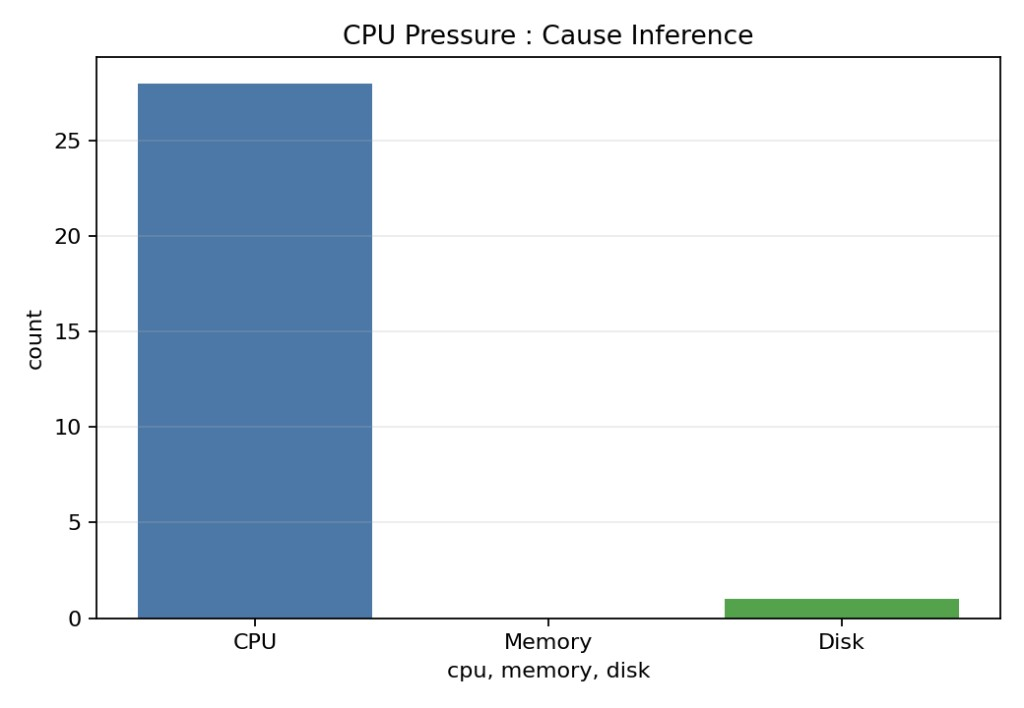
\includegraphics[width=\linewidth]{fig_cause_cpu.png}
  \caption{Cause inference counts under CPU pressure.}
  \label{fig:cause-cpu}
\end{figure}

\begin{figure}[t]
  \centering
  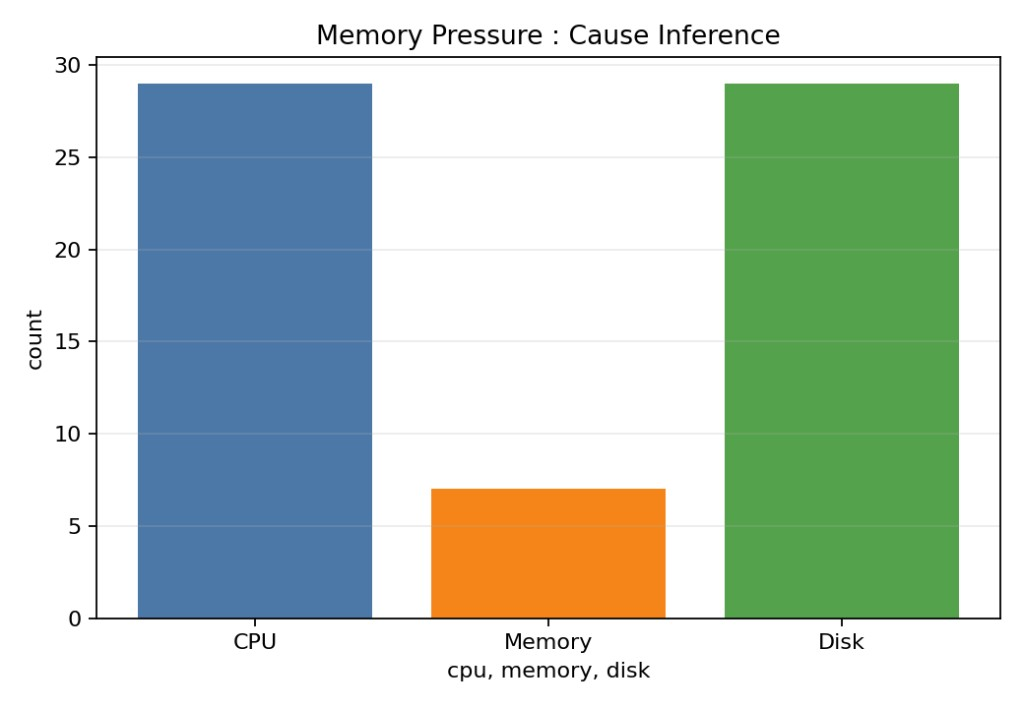
\includegraphics[width=\linewidth]{fig_cause_memory.png}
  \caption{Cause inference counts under memory pressure.}
  \label{fig:cause-memory}
\end{figure}

\begin{figure}[t]
  \centering
  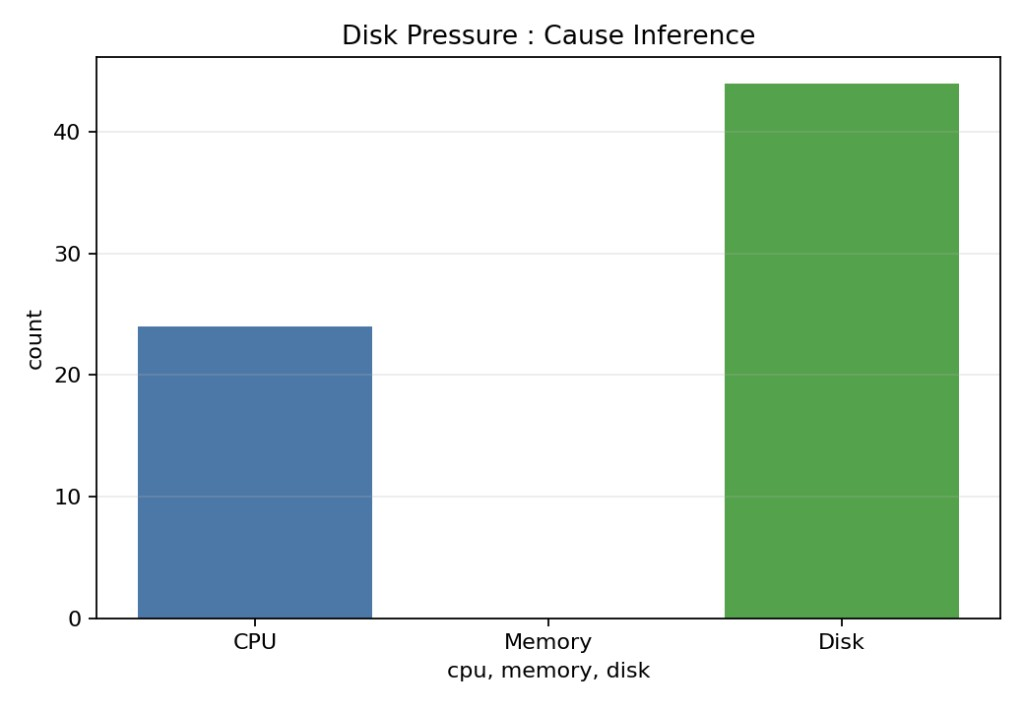
\includegraphics[width=\linewidth]{fig_cause_disk.png}
  \caption{Cause inference counts under disk pressure.}
  \label{fig:cause-disk}
\end{figure}

%------------------------------------------------------------------------------
\subsection{Mitigation timeline against client $p_{95}$ SLO}
\label{subsec:res-mitigation}

Figure~\ref{fig:mitigation-gantt} compares two scripted timelines after a controlled overload that spikes NoSQLBench $p_{95}$ to \textbf{2.09\,s} while the SLO band requires $p_{95}\leq 200$\,ms. Without the UBL-driven mitigation hook, the charted window shows the violation persisting for at least \textbf{90\,s}. With mitigation enabled, latency falls in stages (\textbf{19.3\,s} from 2.09\,s toward 1.0\,s, \textbf{3.24\,s} toward 500\,ms, \textbf{40.13\,s} toward 152\,ms), crosses the SLO by the green marker near \textbf{62.6\,s} cumulative, holds a short stable sub-200\,ms segment (\textbf{5.43\,s}), then enters a \textbf{56\,s} scale-down interval as replicas return from four to three.

The figure is instructive rather than exhaustive: real clusters would interleave repair, stream, and operator approvals. Still, the ordering validates the intended narrative---closed-loop capacity addition can pull client percentiles back inside the band when spare workers exist---while underscoring the multi-tens-of-seconds tail implied by JVM warmup, gossip, and readiness probes (Section~\ref{subsec:challenges-metrics-mitigation}).

\begin{figure*}[t]
  \centering
  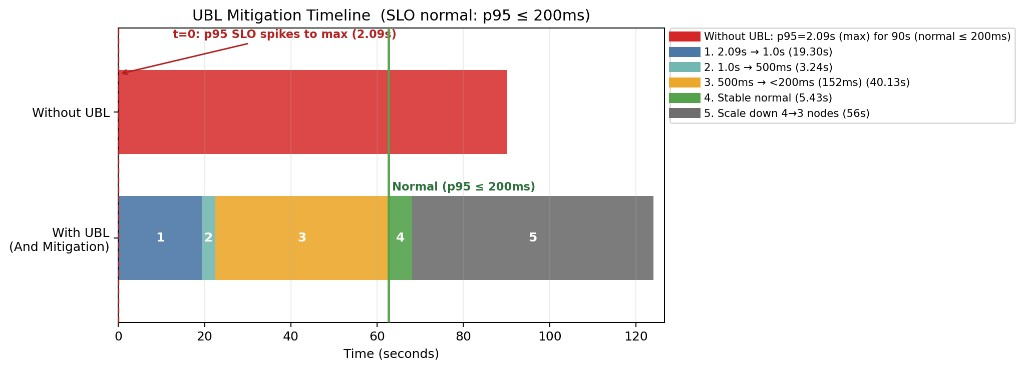
\includegraphics[width=\textwidth]{fig_mitigation_timeline.png}
  \caption{UBL mitigation timeline for NoSQLBench $p_{95}$ relative to a 200\,ms nominal band (annotated run).}
  \label{fig:mitigation-gantt}
\end{figure*}

%------------------------------------------------------------------------------
\subsection{Discussion}
\label{subsec:res-discussion}

Three themes recur across the measurements. First, \textbf{temporal processing matters}: input smoothing and streak debouncing change both ROC shape and measured lead time, so reporting one number without the other is misleading. Second, \textbf{stress labels are not orthogonal to metrics}: cause inference must be interpreted as a ranking heuristic over Tier~A channels, not as ground-truth root-cause isolation. Third, \textbf{mitigation gains are bounded by platform mechanics}: even when detection fires, recovery includes scheduling and Cassandra readiness, so SLO timelines include irreducible tails unrelated to the SOM itself.

Future work in our lab setup would widen the scenario matrix (network partitions, slow disks), tighten memory scenarios so SLO breaches align with memory metrics more cleanly, and explore adaptive $K$ or score-driven debounce instead of fixed streak counts.

%==============================================================================
\section{Limitations and Challenges}
\label{sec:limitations}

This section records practical obstacles encountered while standing up the lab cluster, designing reproducible stress, and closing the loop to SLO-oriented mitigation. The intent is not to criticise individual tools but to document \emph{where} friction arose so future work can budget time and choose platforms accordingly.

%
\subsection{Infrastructure and setup challenges}
\label{subsec:challenges-infra}

\paragraph{Early Multipass-based topology.}
Initial experiments used Multipass VMs on a single physical machine. That topology is attractive for zero-cloud cost and fast iteration, but it concentrates CPU, memory, disk I/O, and network on one host. Contention between the Kubernetes control plane, three Cassandra replicas, monitoring, and stress clients made it difficult to attribute latency spikes to Cassandra behaviour versus hypervisor scheduling. The lesson is qualitative: single-host labs are fine for wiring and demos, but saturated-node effects can dominate results unless resource ceilings are explicitly modelled.

\begin{figure}[t]
  \centering
  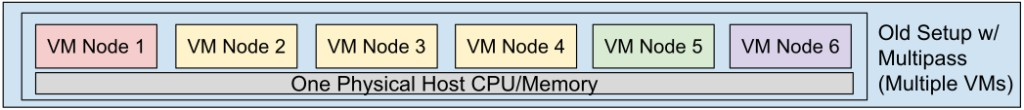
\includegraphics[width=\linewidth]{fig_concept_multipass_legacy.png}
  \caption{Legacy Multipass lab topology (conceptual): several VMs multiplexed on one physical host, sharing CPU and memory capacity.}
  \label{fig:concept-multipass}
\end{figure}

\paragraph{Remote control plane access and CoreDNS (Tailscale).}
When \texttt{kubectl} was driven from a laptop through Tailscale into a home-lab API server, intermittent failures appeared around in-cluster DNS resolution and service discovery. In several cases the failure mode matched a \emph{split-path} problem: the API server was reachable, but UDP/TCP paths needed by CoreDNS or NodePort/ClusterIP routing were blocked or deprioritised by a host or upstream firewall. Symptomatically, pods could schedule yet client Jobs could not resolve \texttt{cassandra.\dots.svc.cluster.local}, or port-forwards would flap. Mitigations in principle include opening the exact ports required by the CNI and kube-proxy path, using \texttt{kubectl} from a bastion inside the same L2/L3 domain as workers, or replacing fragile NAT hairpins with explicit VPN routes. Diagnosis time is substantial because the surface spans OS firewall, cloud security groups (if any), and Kubernetes network policy.

\paragraph{Cloud (AWS) versus lab economics.}
A fully managed or self-managed cluster on AWS would align networking and DNS with well-documented defaults and reduce mystery firewall incidents. The trade-off is lead time (accounts, IAM, VPC design, node groups, storage classes) and recurring cost for long-running fault experiments. For a student or research lab with bursty usage, that overhead pushed the project toward an institutional compute offering instead.

\paragraph{Migration to VCL (Virtual Computing Lab).}
The final platform was VCL: NCSU VMs with clearer network expectations than ad-hoc home routing. Even on VCL, however, \emph{not all} friction disappeared. University-managed images often ship restrictive default firewall policies and conservative outbound rules. Opening NodePorts, LoadBalancer ranges (if used), or Prometheus scrape paths required explicit tickets or self-service rule changes. Similarly, inbound SSH versus in-cluster east-west traffic are governed differently; a rule that allows SSH does not imply pod-to-pod CQL works.

\paragraph{CoreDNS and service discovery on VCL.}
After baseline connectivity was established, residual issues still appeared around DNS caching TTLs, upstream resolver forwarding, and occasional timeouts when the control plane was under load during simultaneous Job churn and StatefulSet rolling events. Operational workarounds included lengthening client driver timeouts during bootstrap, ensuring headless service endpoints were populated before stress start, and verifying that \texttt{ndots} and search-path behaviour in pod resolv.conf matched driver expectations. These are paper cuts individually but compound across a scripted experiment matrix.

\paragraph{Pod affinity and anti-affinity.}
The methodology calls for spreading Cassandra across workers and optionally pinning observability away from data nodes. Expressing that intent in Kubernetes requires careful affinity/anti-affinity rules: \emph{required} rules can make pods unschedulable when the cluster is temporarily smaller than the fault domain count; \emph{preferred} rules allow scheduling but may violate the pedagogical layout. Tuning weights, topology keys, and zone/host labels to match the actual VCL inventory was iterative. StatefulSet ordinals plus hostname-based anti-affinity is standard, yet label drift (e.g., after node replacement) forces playbook updates.

\paragraph{Persistent volume hygiene and node disk pressure.}
Repeated stress runs create SSTables, commitlogs, histostat files, and completed Job logs. Even with TTLs on Jobs, PVCs and hostPath-style provisioners can retain data bound to nodes. Local SSD or small root volumes fill quickly under sustained write-heavy profiles, which in turn triggers kubelet eviction, image garbage collection, and flaky scrapes. A recurring operational task was \emph{deliberate} PVC cleanup between runs: delete bound claims where safe, truncate known directories, or recycle nodes. Without that discipline, mysterious slowdowns in later runs were often plain disk exhaustion rather than algorithmic regression.

%
\subsection{Resource behaviour and stress challenges}
\label{subsec:challenges-stress}

\paragraph{Orthogonality of resource stress.}
Many experiments aim to stress \emph{one} resource channel at a time---for example, push disk I/O while keeping CPU and memory near baseline---so that learner alarms can be attributed to a single family of metrics. Client tools and profile names (\emph{write-heavy}, \emph{disk-oriented}) suggest such isolation, but a sustained CQL write path does not cooperate: the same operations simultaneously consume coordinator and replica CPU (parse, serialize, compress, checksum), grow memtables and buffers in memory, append the commitlog, flush SSTables to disk, and later drive compaction with additional read/write amplification. Workload tuning alone rarely decouples those effects enough for clean ablations. \emph{Isolating} a channel for UBL sensitivity studies therefore required deliberate instrumentation---for example synthetic CPU burn inside a container, cgroup memory limits, or block-device throttling---alongside or instead of relying on stress parameters alone.

\paragraph{Short-lived CPU spikes.}
Inducing a CPU spike visible at Prometheus scrape resolution (e.g., tens of seconds cadence) but short enough to qualify as a brief anomaly is surprisingly finicky. Too short a burn may not register as a sustained elevation in scraped container CPU; too long overlaps the learner's detection horizon and begins to resemble a sustained overload that triggers alarms for the right but experimentally confounding reason. Tuning duration, parallelism, and placement relative to scrape alignment became an empirical loop rather than a one-line parameter.

\paragraph{Memory footprint monotonicity after startup.}
Under Kubernetes, Cassandra's JVM requests memory from the OS and the cgroup controller accounts resident set size conservatively. Observed behaviour matched a well-known pattern: application-reported heap may plateau, while cgroup memory metrics remain high after warmup because pages are not returned to the host at fine granularity, and off-heap/direct buffers add pressure. That complicates memory stress narratives: a post-startup plateau can look like a leak when it is retention policy. Interpreting UBL alarms on memory channels therefore required comparing against GC logs, heap dumps (when feasible), and known Cassandra memory pools rather than raw RSS alone.

\paragraph{Baseline variability and false alarm pressure.}
Even during nominally stable baseline windows, CPU and I/O time series exhibit spikes from garbage collection pauses, minor/major compactions, and periodic background tasks. UBL, being unsupervised and driven by distance-to-manifold scores, can flag these as excursions if the SOM's normal model is too tight or the streak debouncer is too short. This is a methodological limitation: \emph{operational normality} for Cassandra includes bursty housekeeping. Separating interesting stress from housekeeping motivated longer baselines, score smoothing, and evaluation windows $W$ that tolerate brief benign spikes.

%
\subsection{Metrics and mitigation challenges}
\label{subsec:challenges-metrics-mitigation}

\paragraph{SLO signal extraction from cassandra-stress logs.}
An early approach derived p95/p99 style SLO proxies by scraping or parsing \texttt{cassandra-stress} textual output from ephemeral Job pods. Problems stacked quickly: stress tools emit high-volume logs; multiple threads interleave lines; pods restart and lose local log history; regex parsers are brittle across version strings and locale formatting. End-to-end latency from log ship to metric availability was high enough to lag alarms and distort lead-time studies.

\paragraph{NoSQLBench as the cleaner path.}
Switching client-side latency reporting to NoSQLBench's structured outputs (notably CSV-oriented histostat series exposed via a metrics sidecar) reduced parsing complexity and improved alignment with Prometheus scrape models. The conceptual point is that \emph{first-class metrics} beat \emph{log archaeology} for closed-loop experiments.

\paragraph{Cold-start latency after scale-out.}
Even when mitigation correctly detects sustained SLO violation and increases StatefulSet replicas, a new Cassandra pod is not immediately queryable. Bootstrapping, JVM warmup, gossip convergence, and readiness probes routinely consumed on the order of twenty seconds in lab conditions (exact timing depends on image, CPU, and IO). Kubernetes does not provide a native hot standby CQL replica that instantaneously absorbs load; capacity appears as a schedulable pod that must join the ring. Therefore mitigation experiments must either (a) bake cooldown and evaluation delays into timelines, or (b) treat post-scale SLO recovery as a two-phase phenomenon: \emph{scheduling} plus \emph{service readiness}.

\paragraph{Implication for evaluation.}
Lead time and \texttt{Ntp}/\texttt{Nfn} definitions assume timestamps for alarms and breaches are comparable and well clock-synchronised. Mitigation scripts that poll Prometheus with coarse intervals can miss sub-minute recovery dynamics, overstating violation duration or understating recovery. Reporting should state scrape cadence and probe semantics alongside mitigation outcomes.

%

\section{Distribution of Work}
\subsection{Aum}
Stress (Cassandra Stress , No SQL Bench), Mitigation, Old Multipass Kubernetes setup, Networking setup, Tailscale Experiments

\subsection{Darsh}
UBL (training and inference setup), hyperparameter tuning, Evaluation metrics implementation


\subsection{Dilip}
Current  VCL 3 node setup (k3s , kubernetes), AWS setup, Networking setup, Monitoring Setup (Prom + Grafana)

\subsection{ALL}
Integration, Experiments, Evaluation, Documentation



% \section{Typefaces}

% The \verb|acmart| document class requires the use of the
% Libertine typeface family. Your \TeX\ installation should include
% this set of packages. Please do not substitute other typefaces. The
% \verb|lmodern| and \verb|ltimes| packages should not be used,
% as they will override the built-in typeface families.

% \section{Title Information}

% The title of your work should use capital letters appropriately -
% \url{https://capitalizemytitle.com/} has useful rules for
% capitalization. Use the {\verb|title|} command to define the title of
% your work. If your work has a subtitle, define it with the
% {\verb|subtitle|} command.  Do not insert line breaks in your title.

% If your title is lengthy, you must define a short version to be used
% in the page headers, to prevent overlapping text. The \verb|title|
% command has a short title parameter:
% \begin{verbatim}
%   \title[short title]{full title}
% \end{verbatim}

% \section{Authors and Affiliations}

% Each author must be defined separately for accurate metadata
% identification.  As an exception, multiple authors may share one
% affiliation. Authors' names should not be abbreviated; use full first
% names wherever possible. Include authors' e-mail addresses whenever
% possible.

% Grouping authors' names or e-mail addresses, or providing an e-mail
% alias, as shown below, is not acceptable:
% \begin{verbatim}
%   \author{Brooke Aster, David Mehldau}
%   \email{dave,judy,steve@university.edu}
%   \email{firstname.lastname@phillips.org}
% \end{verbatim}

% The \verb|authornote| and \verb|authornotemark| commands allow a note
% to apply to multiple authors  for example, if the first two authors
% of an article contributed equally to the work.

% If your author list is lengthy, you must define a shortened version of
% the list of authors to be used in the page headers, to prevent
% overlapping text. The following command should be placed just after
% the last \verb|\author{}| definition:
% \begin{verbatim}
%   \renewcommand{\shortauthors}{McCartney, et al.}
% \end{verbatim}
% Omitting this command will force the use of a concatenated list of all
% of the authors' names, which may result in overlapping text in the
% page headers.

% The article template's documentation, available at
% \url{https://www.acm.org/publications/proceedings-template}, has a
% complete explanation of these commands and tips for their effective
% use.

% Note that authors' addresses are mandatory for journal articles.

% \section{Rights Information}

% Authors of any work published by ACM will need to complete a rights
% form. Depending on the kind of work, and the rights management choice
% made by the author, this may be copyright transfer, permission,
% license, or an OA (open access) agreement.

% Regardless of the rights management choice, the author will receive a
% copy of the completed rights form once it has been submitted. This
% form contains \LaTeX\ commands that must be copied into the source
% document. When the document source is compiled, these commands and
% their parameters add formatted text to several areas of the final
% document:
% \begin{itemize}
% \item the ACM Reference Format text on the first page.
% \item the rights management text on the first page.
% \item the conference information in the page header(s).
% \end{itemize}

% Rights information is unique to the work; if you are preparing several
% works for an event, make sure to use the correct set of commands with
% each of the works.

% The ACM Reference Format text is required for all articles over one
% page in length, and is optional for one-page articles (abstracts).

% \section{CCS Concepts and User-Defined Keywords}

% Two elements of the acmart document class provide powerful
% taxonomic tools for you to help readers find your work in an online
% search.

% The ACM Computing Classification System 
% \url{https://www.acm.org/publications/class-2012}  is a set of
% classifiers and concepts that describe the computing
% discipline. Authors can select entries from this classification
% system, via \url{https://dl.acm.org/ccs/ccs.cfm}, and generate the
% commands to be included in the \LaTeX\ source.

% User-defined keywords are a comma-separated list of words and phrases
% of the authors' choosing, providing a more flexible way of describing
% the research being presented.

% CCS concepts and user-defined keywords are required for for all
% articles over two pages in length, and are optional for one- and
% two-page articles (or abstracts).

% \section{Sectioning Commands}

% Your work should use standard \LaTeX\ sectioning commands:
% \verb|\section|, \verb|\subsection|, \verb|\subsubsection|,
% \verb|\paragraph|, and \verb|\subparagraph|. The sectioning levels up to
% \verb|\subsusection| should be numbered; do not remove the numbering
% from the commands.

% Simulating a sectioning command by setting the first word or words of
% a paragraph in boldface or italicized text is {\bfseries not allowed.}

% Below are examples of sectioning commands.

% \subsection{Subsection}
% \label{sec:subsection}

% This is a subsection.

% \subsubsection{Subsubsection}
% \label{sec:subsubsection}

% This is a subsubsection.

% \paragraph{Paragraph}

% This is a paragraph.

% \subparagraph{Subparagraph}

% This is a subparagraph.

% \section{Tables}

% The \verb|acmart| document class includes the \verb|booktabs|
% package  \url{https://ctan.org/pkg/booktabs}  for preparing
% high-quality tables.

% Table captions are placed {\itshape above} the table.

% Because tables cannot be split across pages, the best placement for
% them is typically the top of the page nearest their initial cite.  To
% ensure this proper floating placement of tables, use the
% environment \textbf{table} to enclose the table's contents and the
% table caption.  The contents of the table itself must go in the
% \textbf{tabular} environment, to be aligned properly in rows and
% columns, with the desired horizontal and vertical rules.  Again,
% detailed instructions on \textbf{tabular} material are found in the
% \textit{\LaTeX\ User's Guide}.

% Immediately following this sentence is the point at which
% Table~\ref{tab:freq} is included in the input file; compare the
% placement of the table here with the table in the printed output of
% this document.

% \begin{table}
%   \caption{Frequency of Special Characters}
%   \label{tab:freq}
%   \begin{tabular}{ccl}
%     \toprule
%     Non-English or Math&Frequency&Comments\\
%     \midrule
%     \O & 1 in 1,000& For Swedish names\\
%     $\pi$ & 1 in 5& Common in math\\
%     \$ & 4 in 5 & Used in business\\
%     $\Psi^2_1$ & 1 in 40,000& Unexplained usage\\
%   \bottomrule
% \end{tabular}
% \end{table}

% To set a wider table, which takes up the whole width of the page's
% live area, use the environment \textbf{table*} to enclose the table's
% contents and the table caption.  As with a single-column table, this
% wide table will float to a location deemed more
% desirable. Immediately following this sentence is the point at which
% Table~\ref{tab:commands} is included in the input file; again, it is
% instructive to compare the placement of the table here with the table
% in the printed output of this document.

% \begin{table*}
%   \caption{Some Typical Commands}
%   \label{tab:commands}
%   \begin{tabular}{ccl}
%     \toprule
%     Command &A Number & Comments\\
%     \midrule
%     \texttt{{\char'134}author} & 100& Author \\
%     \texttt{{\char'134}table}& 300 & For tables\\
%     \texttt{{\char'134}table*}& 400& For wider tables\\
%     \bottomrule
%   \end{tabular}
% \end{table*}

% Always use midrule to separate table header rows from data rows, and
% use it only for this purpose. This enables assistive technologies to
% recognise table headers and support their users in navigating tables
% more easily.

% \section{Math Equations}
% You may want to display math equations in three distinct styles:
% inline, numbered or non-numbered display.  Each of the three are
% discussed in the next sections.

% \subsection{Inline (In-text) Equations}
% A formula that appears in the running text is called an inline or
% in-text formula.  It is produced by the \textbf{math} environment,
% which can be invoked with the usual
% \texttt{{\char'134}begin\,\ldots{\char'134}end} construction or with
% the short form \texttt{\$\,\ldots\$}. You can use any of the symbols
% and structures, from $\alpha$ to $\omega$, available in
% \LaTeX~\cite{Lamport:LaTeX}; this section will simply show a few
% examples of in-text equations in context. Notice how this equation:
% \begin{math}
%   \lim_{n\rightarrow \infty}x=0
% \end{math},
% set here in in-line math style, looks slightly different when
% set in display style.  (See next section).

% \subsection{Display Equations}
% A numbered display equationone set off by vertical space from the
% text and centered horizontallyis produced by the \textbf{equation}
% environment. An unnumbered display equation is produced by the
% \textbf{displaymath} environment.

% Again, in either environment, you can use any of the symbols and
% structures available in \LaTeX\@; this section will just give a couple
% of examples of display equations in context.  First, consider the
% equation, shown as an inline equation above:
% \begin{equation}
%   \lim_{n\rightarrow \infty}x=0
% \end{equation}
% Notice how it is formatted somewhat differently in
% the \textbf{displaymath}
% environment.  Now, we'll enter an unnumbered equation:
% \begin{displaymath}
%   \sum_{i=0}^{\infty} x + 1
% \end{displaymath}
% and follow it with another numbered equation:
% \begin{equation}
%   \sum_{i=0}^{\infty}x_i=\int_{0}^{\pi+2} f
% \end{equation}
% just to demonstrate \LaTeX's able handling of numbering.

% \section{Figures}

% The \verb|figure| environment should be used for figures. One or
% more images can be placed within a figure. If your figure contains
% third-party material, you must clearly identify it as such, as shown
% in the example below.
% \begin{figure}[h]
%   \centering
%   \includegraphics[width=\linewidth]{sample-franklin}
%   \caption{1907 Franklin Model D roadster. Photograph by Harris \&
%     Ewing, Inc. [Public domain], via Wikimedia
%     Commons. (\url{https://goo.gl/VLCRBB}).}
%   \Description{A woman and a girl in white dresses sit in an open car.}
% \end{figure}

% Your figures should contain a caption which describes the figure to
% the reader.

% Figure captions are placed {\itshape below} the figure.

% Every figure should also have a figure description unless it is purely
% decorative. These descriptions convey what’s in the image to someone
% who cannot see it. They are also used by search engine crawlers for
% indexing images, and when images cannot be loaded.

% A figure description must be unformatted plain text less than 2000
% characters long (including spaces).  {\bfseries Figure descriptions
%   should not repeat the figure caption – their purpose is to capture
%   important information that is not already provided in the caption or
%   the main text of the paper.} For figures that convey important and
% complex new information, a short text description may not be
% adequate. More complex alternative descriptions can be placed in an
% appendix and referenced in a short figure description. For example,
% provide a data table capturing the information in a bar chart, or a
% structured list representing a graph.  For additional information
% regarding how best to write figure descriptions and why doing this is
% so important, please see
% \url{https://www.acm.org/publications/taps/describing-figures/}.

% \subsection{The Teaser Figure}

% A teaser figure is an image, or set of images in one figure, that
% are placed after all author and affiliation information, and before
% the body of the article, spanning the page. If you wish to have such a
% figure in your article, place the command immediately before the
% \verb|\maketitle| command:
% \begin{verbatim}
%   \begin{teaserfigure}
%     \includegraphics[width=\textwidth]{sampleteaser}
%     \caption{figure caption}
%     \Description{figure description}
%   \end{teaserfigure}
% \end{verbatim}

% \section{Citations and Bibliographies}

% The use of \BibTeX\ for the preparation and formatting of one's
% references is strongly recommended. Authors' names should be complete
%  use full first names (Donald E. Knuth) not initials
% (D. E. Knuth)  and the salient identifying features of a
% reference should be included: title, year, volume, number, pages,
% article DOI, etc.

% The bibliography is included in your source document with these two
% commands, placed just before the \verb|\end{document}| command:
% \begin{verbatim}
%   \bibliographystyle{ACM-Reference-Format}
%   \bibliography{bibfile}
% \end{verbatim}
% where \verb|bibfile| is the name, without the \verb|.bib|
% suffix, of the \BibTeX\ file.

% Citations and references are numbered by default. A small number of
% ACM publications have citations and references formatted in the
% author year style; for these exceptions, please include this
% command in the {\bfseries preamble} (before the command
% \verb|\begin{document}|) of your \LaTeX\ source:
% \begin{verbatim}
%   \citestyle{acmauthoryear}
% \end{verbatim}


%   Some examples.  A paginated journal article \cite{Abril07}, an
%   enumerated journal article \cite{Cohen07}, a reference to an entire
%   issue \cite{JCohen96}, a monograph (whole book) \cite{Kosiur01}, a
%   monograph/whole book in a series (see 2a in spec. document)
%   \cite{Harel79}, a divisible-book such as an anthology or compilation
%   \cite{Editor00} followed by the same example, however we only output
%   the series if the volume number is given \cite{Editor00a} (so
%   Editor00a's series should NOT be present since it has no vol. no.),
%   a chapter in a divisible book \cite{Spector90}, a chapter in a
%   divisible book in a series \cite{Douglass98}, a multi-volume work as
%   book \cite{Knuth97}, a couple of articles in a proceedings (of a
%   conference, symposium, workshop for example) (paginated proceedings
%   article) \cite{Andler79, Hagerup1993}, a proceedings article with
%   all possible elements \cite{Smith10}, an example of an enumerated
%   proceedings article \cite{VanGundy07}, an informally published work
%   \cite{Harel78}, a couple of preprints \cite{Bornmann2019,
%     AnzarootPBM14}, a doctoral dissertation \cite{Clarkson85}, a
%   master's thesis: \cite{anisi03}, an online document / world wide web
%   resource \cite{Thornburg01, Ablamowicz07, Poker06}, a video game
%   (Case 1) \cite{Obama08} and (Case 2) \cite{Novak03} and \cite{Lee05}
%   and (Case 3) a patent \cite{JoeScientist001}, work accepted for
%   publication \cite{rous08}, 'YYYYb'-test for prolific author
%   \cite{SaeediMEJ10} and \cite{SaeediJETC10}. Other cites might
%   contain 'duplicate' DOI and URLs (some SIAM articles)
%   \cite{Kirschmer:2010:AEI:1958016.1958018}. Boris / Barbara Beeton:
%   multi-volume works as books \cite{MR781536} and \cite{MR781537}. A
%   presentation~\cite{Reiser2014}. An article under
%   review~\cite{Baggett2025}. A
%   couple of citations with DOIs:
%   \cite{2004:ITE:1009386.1010128,Kirschmer:2010:AEI:1958016.1958018}. Online
%   citations: \cite{TUGInstmem, Thornburg01, CTANacmart}.
%   Artifacts: \cite{R} and \cite{UMassCitations}.

% \section{Acknowledgments}

% Identification of funding sources and other support, and thanks to
% individuals and groups that assisted in the research and the
% preparation of the work should be included in an acknowledgment
% section, which is placed just before the reference section in your
% document.

% This section has a special environment:
% \begin{verbatim}
%   \begin{acks}
%   ...
%   \end{acks}
% \end{verbatim}
% so that the information contained therein can be more easily collected
% during the article metadata extraction phase, and to ensure
% consistency in the spelling of the section heading.

% Authors should not prepare this section as a numbered or unnumbered {\verb|\section|}; please use the {\verb|acks|} environment.

% \section{Appendices}

% If your work needs an appendix, add it before the
% \verb|\end{document}| command at the conclusion of your source
% document.

% Start the appendix with the \verb|appendix| command:
% \begin{verbatim}
%   \appendix
% \end{verbatim}
% and note that in the appendix, sections are lettered, not
% numbered. This document has two appendices, demonstrating the section
% and subsection identification method.

% \section{Multi-language papers}

% Papers may be written in languages other than English or include
% titles, subtitles, keywords and abstracts in different languages (as a
% rule, a paper in a language other than English should include an
% English title and an English abstract).  Use \verb|language=...| for
% every language used in the paper.  The last language indicated is the
% main language of the paper.  For example, a French paper with
% additional titles and abstracts in English and German may start with
% the following command
% \begin{verbatim}
% \documentclass[sigconf, language=english, language=german,
%                language=french]{acmart}
% \end{verbatim}

% The title, subtitle, keywords and abstract will be typeset in the main
% language of the paper.  The commands \verb|\translatedXXX|, \verb|XXX|
% begin title, subtitle and keywords, can be used to set these elements
% in the other languages.  The environment \verb|translatedabstract| is
% used to set the translation of the abstract.  These commands and
% environment have a mandatory first argument: the language of the
% second argument.  See \verb|sample-sigconf-i13n.tex| file for examples
% of their usage.

% \section{SIGCHI Extended Abstracts}

% The \verb|sigchi-a| template style (available only in \LaTeX\ and
% not in Word) produces a landscape-orientation formatted article, with
% a wide left margin. Three environments are available for use with the
% \verb|sigchi-a| template style, and produce formatted output in
% the margin:
% \begin{description}
% \item[\texttt{sidebar}:]  Place formatted text in the margin.
% \item[\texttt{marginfigure}:] Place a figure in the margin.
% \item[\texttt{margintable}:] Place a table in the margin.
% \end{description}

% %%
% %% The acknowledgments section is defined using the "acks" environment
% %% (and NOT an unnumbered section). This ensures the proper
% %% identification of the section in the article metadata, and the
% %% consistent spelling of the heading.
% \begin{acks}
% To Robert, for the bagels and explaining CMYK and color spaces.
% \end{acks}

% %%
% %% The next two lines define the bibliography style to be used, and
% %% the bibliography file.

\bibliographystyle{ACM-Reference-Format}
\bibliography{software}


% %%
% %% If your work has an appendix, this is the place to put it.
\appendix
\section*{Appendix: notation summary}
\begin{tabular}{@{}ll@{}}
\toprule
Symbol & Meaning \\
\midrule
$\mathbf{x}(t)$ & raw aggregated Tier~A feature vector at time $t$ \\
$\mathbf{z}(t)$ & normalised feature vector \\
$(r^\star,c^\star)$ & BMU coordinates \\
$s(t)$ & anomaly score (area-map based) \\
$\tau$ & alarm threshold on $s(t)$ \\
$L$ & streak length for debouncing \\
$W$ & pending/lead-time evaluation window \\
$\theta$ & SLO latency threshold (ms) \\
\bottomrule
\end{tabular}

% \section{Research Methods}

% \subsection{Part One}

% Lorem ipsum dolor sit amet, consectetur adipiscing elit. Morbi
% malesuada, quam in pulvinar varius, metus nunc fermentum urna, id
% sollicitudin purus odio sit amet enim. Aliquam ullamcorper eu ipsum
% vel mollis. Curabitur quis dictum nisl. Phasellus vel semper risus, et
% lacinia dolor. Integer ultricies commodo sem nec semper.

% \subsection{Part Two}

% Etiam commodo feugiat nisl pulvinar pellentesque. Etiam auctor sodales
% ligula, non varius nibh pulvinar semper. Suspendisse nec lectus non
% ipsum convallis congue hendrerit vitae sapien. Donec at laoreet
% eros. Vivamus non purus placerat, scelerisque diam eu, cursus
% ante. Etiam aliquam tortor auctor efficitur mattis.

% \section{Online Resources}

% Nam id fermentum dui. Suspendisse sagittis tortor a nulla mollis, in
% pulvinar ex pretium. Sed interdum orci quis metus euismod, et sagittis
% enim maximus. Vestibulum gravida massa ut felis suscipit
% congue. Quisque mattis elit a risus ultrices commodo venenatis eget
% dui. Etiam sagittis eleifend elementum.

% Nam interdum magna at lectus dignissim, ac dignissim lorem
% rhoncus. Maecenas eu arcu ac neque placerat aliquam. Nunc pulvinar
% massa et mattis lacinia.

\end{document}
\endinput
%%
%% End of file `sample-sigconf-authordraft.tex'.

